\documentclass[fontsize=12bp, paper=a4]{scrarticle}
\usepackage[utf8]{inputenc}
\usepackage[english,main=serbian]{babel}
\usepackage[left=2cm, right=2cm, top=3cm, bottom=3cm]{geometry}
\usepackage[automark]{scrlayer-scrpage}
\usepackage{ragged2e}
\usepackage{amsmath}
\usepackage{mathabx}
\usepackage[colorlinks=true,linkcolor=black,anchorcolor=black,citecolor=black,filecolor=black,menucolor=black,runcolor=black,urlcolor=black]{hyperref}
\usepackage{graphicx}
\usepackage{wrapfig}
\usepackage{amssymb}
\usepackage{listings}
\usepackage{xcolor}
\usepackage{csquotes}
\usepackage{booktabs}
\usepackage{cancel}

%\usepackage[backend=biber, style=numeric]{biblatex}
% kompilirati sa pdflatex-om!
\justifying
%
\definecolor{codegreen}{rgb}{0,0.6,0}
\definecolor{codegray}{rgb}{0.5,0.5,0.5}
\definecolor{codepurple}{rgb}{0.58,0,0.82}
\definecolor{backcolour}{rgb}{0.95,0.95,0.92}

\lstdefinestyle{mystyle}{
    backgroundcolor=\color{backcolour},   
    commentstyle=\color{codegreen},
    keywordstyle=\color{magenta},
    numberstyle=\tiny\color{codegray},
    stringstyle=\color{codepurple},
    basicstyle=\ttfamily\footnotesize,
    breakatwhitespace=false,         
    breaklines=true,                 
    captionpos=b,                    
    keepspaces=true,                 
    numbers=left,                    
    numbersep=5pt,                  
    showspaces=false,                
    showstringspaces=false,
    showtabs=false,                  
    tabsize=2
}

\lstset{style=mystyle}

\renewcommand\lstlistingname{Implementacija}
\renewcommand\lstlistlistingname{Implementacija}

%

\graphicspath{ {./images/} }

%

\title{Seminarski rad} 
\subtitle{iz predmeta Teorijske osnove veštačke inteligencije}

\begin{document}

\begin{titlepage}
    \vspace{\stretch{1}}
    
    \begin{center}
        
        \vspace*{8cm}
        
        \large{Univerzitet u Kragujevcu}
        
        \vspace*{1cm}

        {\bfseries \LARGE Domaći zadatak}
        
        \large{iz predmeta Sistem za podršku odlučivanju}
        
        \vspace*{1cm}
        \large{Tema:}

        \Large{Teorijski izveštaj o klasifikacionim algoritmima sa nadgledanim učenjem}


        \vspace*{2cm}
    \end{center}
    \hfill{\parbox[s]{8cm}{

    mentori: 
    \begin{tabular}{l}
        \\
        \\
        Ognjen Pavić, \\
        prof. dr. Tijana Geroski, \\
        prof. dr. Nenad Filipović 
    \end{tabular}
    
    student: \begin{tabular}{l}
        Željko Simić 3vi/2023
    \end{tabular}
    }}

    \hspace*{\fill} 

    \vspace*{2cm}

    \begin{center}
        Kragujevac 2024.
    \end{center}
\end{titlepage}


\setcounter{page}{1}
\justifying
\linespread{1}
\cfoot[\pagemark]{\pagemark}
\ofoot[]{}
\ohead[]{Željko Simić 3vi/2023}
\chead[]{}
\ihead[]{Univerzitet u Kragujevcu}
%
\justify

\section{Uvod}
\subsection{Opis procesa učenja\cite{supervised}}
Problem obuke obuhvata skupinu $n$ uzoraka podataka i time se pokušava predvideti svojstvo nepoznatih podataka. Ako svaki uzorak ponaosob je više nego 1 unos, npr., multidimenzionalni unos, može se reći da ima više atributa ili features-a.
\\
\justifying

Problemi obuke potpadaju u nekoliko kategorija:
\begin{itemize}
    \item \textit{Nenadgledajuće učenje (nije tema ovog rada)} - obuka podacima sastoji se u unosu više vektora $x$ bez ikakvih uparenih ciljnih vrednosti. Cilj je otkriti pripadnost grupi po sličnosti naspram drugih vektora (klasterizacija), ili po raspodeli podataka unutar prostora ulaznih podataka (procena gustine), ili po projekciji podataka višedimenzionog prostora na manje dimenzioni shodnom za vizuelizaciju.
    
    \item \textit{Delimično nadgledano učenje (nije tema ovog rada)\cite{semi}} - situacija gde skup podataka namenjen za obuku ima poneki uzorak koji nije uparen sa ciljanom vrednošću, gde se zarad adekvatnijeg previđanja boljom generalizacijom i distribucijom koriste ciljanom vrednošću nenaznačeni uzorci.
    
    \item \textit{Podsticajuće učenje (nije tema ovog rada)\cite{rl}} - opšti okvir rada gde se vrši obuka \textit{agenata} (tj. algoritma obuke) težeći da se obuče da vrše akcije u zadatom \textit{okruženju} (tj. problema za rešavanje) zarad najboljeg mogućeg slučaja nagrađivanja. 

    \item \textit{\textbf{Nadgledano učenje}} - gde se skup podataka sa prikazanim primerom na slici 1. prilaže sa dodatnim atributima po kojim će se predviđanje usmeravati (klasa za svaki od uzoraka, labela). Sastoji se od 2 načina rada (gde samo jednog obrađujemo):
    \begin{itemize}
        \item \textit{Regresija (delimično nije tema rada)} - gde željeni izlaz u priloženom skupu podataka se izražava kao jedna ili više kontinualnih promenljivih, a zadatak predviđanja da nepoznatim ulazima uzorka se naziva regresijom.
        \item \textit{\textbf{Klasifikacija}} - uzorci mogu da pripadaju dvema (binarna klasifikacija) ili više klasa (višeklasna klasifikacija) i želimo ustanoviti kako bi se predviđanje klasa za nenaznačene podatke vršilo uz pomoć već klasama naznačenih podataka. Način da se sagleda klasifikacija je kao diskretni (suprotno kontinualnom) oblik nadgledane obuke gde od ograničenog broja kategorija za svaki od n uzoraka se namerava dodeliti tačna klasa ili kategorija.
        \begin{figure}[h!]
            \centering
            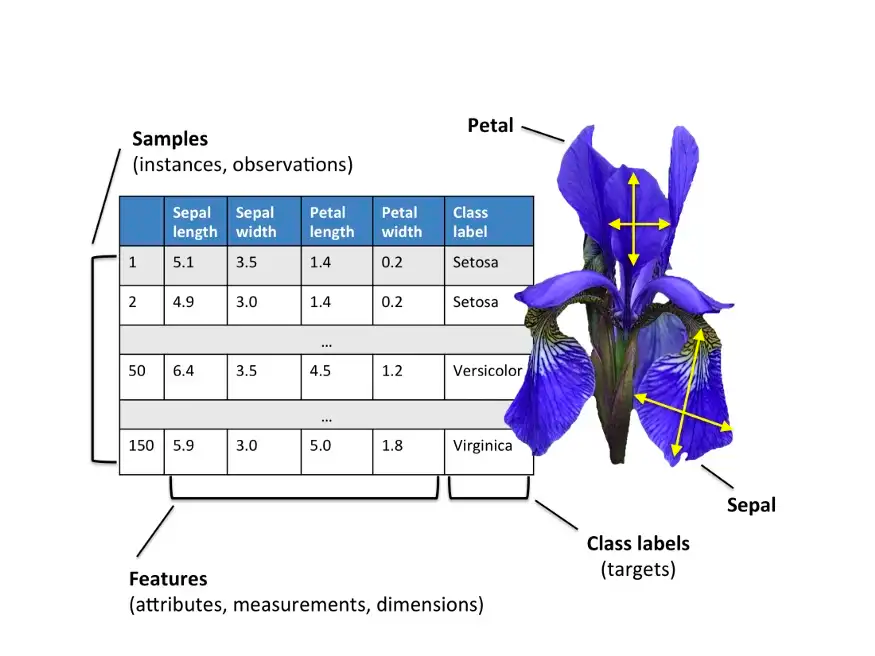
\includegraphics[width=0.75\textwidth]{image.png}
            \caption{\centering Primer višeklasnog skupa podataka - Iris flower, sa atributima Sepal length, Sepal width, Petal length, Petal width i atributom klase \textit {Class label} u posebnih 150 uzoraka.}
        \end{figure}

    \end{itemize}    
\end{itemize}     

\subsubsection{Trening skup i test skup}
Mašinsko učenje se sačinjava od poduhvata gde se vrši obuka uz svojstva jednog skupa podataka, a vrši testiranje svojstvima uz pomoć nekih drugih skupova podataka. Uobičajena praksa u mašinskom učenju je da se vrši evaluacija algoritma uz podelu skupa podataka na 2 dela. Gde je jedan deo namenjen za obuku (trening skup), a drugi za testiranje (test skup).

\subsubsection{Multiclass vs. multilabel obuka}
Kada se koriste multiklasni klasifikatori, zadaci obuka i predviđanja se izvršavaju tako da zavise od formata podataka ciljanih vrednosti. 1D niz višeklasna labela skupljenih svih uzoraka je moguće navesti da radi \textit{multiklasna predviđanja}. Ciljane vrednosti je moguće mapirati tako da se konvertuju u binarni zapis, tj. niz sastojan od binarnih cifara tako da skup uzoraka ima ciljane vrednosti kao 2d niz i nakon obuke, za obavljana predviđanja smatra se da su \textit{multilabel predviđanja}. Takođe je moguće da ciljana vrednost ima niz više labela (skupljeno po svim uzorcima ciljana vrednost biva 2d niz) za svaki uzorak pri obuci i kasnije naspram toga vršiti predviđanja.


% TODO Problem nadgledane klasifikacije moguće je najpogodnije uočiti pri prepoznavanju rukom napisanih brojeva, tako da se cilja da se dodeli svaki pojedinačno vektor nekoj od konačno prebrojivih diskretnih kategorija. 
\subsubsection{Popularni algoritmi za klasifikaciju\cite{algs}}
\justifying

\begin{itemize}
    \item \textbf{Logistička regresija} - je algoritam nalik linearnoj regresiji samo što umesto ciljana vrednost da bude neki broj, ona biva neka binarna vrednost ('Da'/'Ne', 0/1). Iako se naziva regresijom ona vrši klasifikaciju na osnovu regresije.
    \item \textbf{K-Najbližih suseda (kNN)} - najjednostavniji klasifikatorni algoritam korišćen da uoči uzorke (npr. Euklidskoj distanci) podeljene po raznovrsnim klasama da bi predvideli klasifikaciju novonastalog uzorka.
    \item \textbf{Mašina potpornih vektora (SVM)} - korišćen u oba tipa nadgledanog učenja i zasnovan na konceptu ravni odlučivanja (hiperravni) koje ističu ograničenja odlučivanja, tj. dele skup uzoraka na pripadnost u različitim klasama. 
    \item \textbf{Naivni Bajes} - zasnovan na Bajesovoj teoremi uz više nezavisnih pretpostavki među predviđačima.
    \item \textbf{Stablo odlučivanja} -  korišćen u oba tipa nadgledanog učenja u obliku strukture stabla. Razbija svakom iteracijom skup podataka u sve manje podskupove, dok pritom je stablo odlučivanja inkrementalno razvijeno. 
    \item \textit{Metodi ansambla} - sadrže nekolicinu nadzirajućih modela obuke koji su svaki za sebe posebno obučeni i rezultati su objedinjeni na raznolike načine da bi se dobilo kranje predviđanje. Neki od algoritama ovog tipa su:
    \begin{itemize}
        \item \textbf{Klasifikacija slučajnih šuma} - algoritam zasnovan na bagging/bootstrap agregaciji koja eliminiše problem overfitting-a, poboljšava tačnost i smanjuje bias (pristrasnost).
        \item \textit{Klasifikacija boost-ovanog gradijenta (neće biti obrađivan)} - objedinjava slabe obučivače, primarno da bi izbegao bias pri predviđanju. Umesto da se radi bagging - gomilanje predviđaća, radi se boosting gde se radi ''slivanje'' iz jednog obučivača u drugi.
    \end{itemize}
\end{itemize}
U sledećim sekcijama biće obrađivani pomenuti algoritmi.
\newpage

\section{Teorijske osnove i metodologija}
\subsection{Logistička regresija}
Predstavlja se kao linearni model pre za klasifikaciju, nego za regresiju. Poznata je u nekim literaturama kao:
\begin{itemize}
    \item logit regresija - predstavljena (i vizuelizovana na slici 2.) kao inverz sigmoidne-logističke funkcije, gde po verovatnoći $p$, važi $logit(p) = log(\frac{p}{1-p})$\cite{logit}, tzv. logaritam neobičnosti - odnos verovatnoća da će se događaj desiti i da se neće desiti; moguće je kasnije svesti na oblik linearne kombinacije $logit(p) = \beta_0 + \beta_1X_1 + \beta_2X_2 + ... + \beta_kX_k$\cite{logit2}; prikazana na slici 3.;
    \begin{figure}[h!]
        \centering
        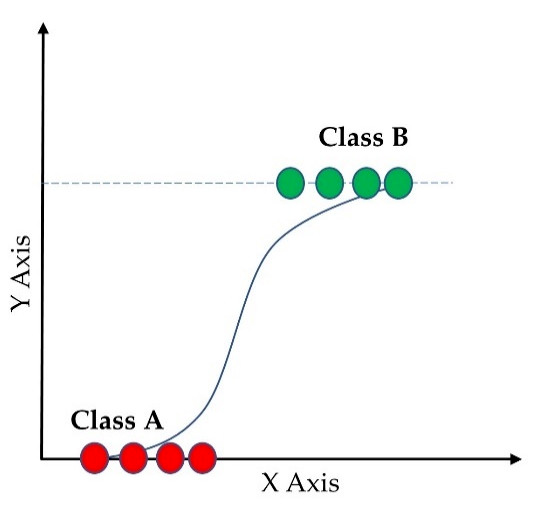
\includegraphics[width=0.35\textwidth]{image-5.png}
        \caption{Rad logističke regresije za klasifikaciju uzoraka A i B.}
    \end{figure}
    \begin{figure}[h!]
        \centering
        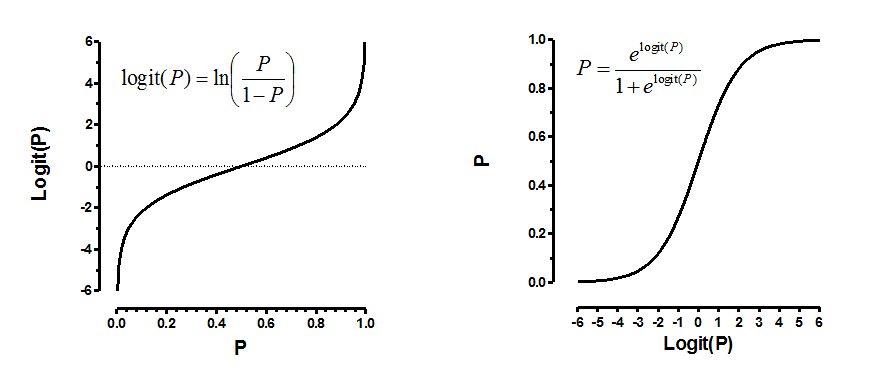
\includegraphics[width=0.75\textwidth]{image-1.png}
        \caption{Grafici logit i sigmoidne funkcije.}
    \end{figure}
    \item klasifikacija maksimuma-entropije - što veće neizvesnosti/raznolikosti u skupu podataka\cite{entropy} po verovatnoći da se desi događaj $P_i$ slučajnog odabira uzorka klase $i$, gde važi $E = - \sum^N_{i=1}P_i * log_2(P_i)$, prikaz na slici 4.;
    \begin{figure}[h!]
        \centering
        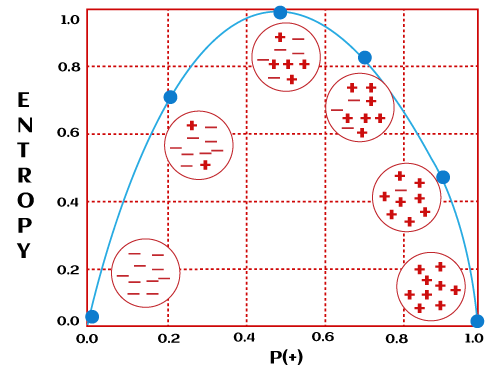
\includegraphics[width=0.35\textwidth]{image-2.png}
        \caption{Ilustracija putem grafika funkcije entropije.}
    \end{figure}
    \item iliti log-linearni klasifikator - koji za razliku od linearnog modela, maločas pomenutog, se zasniva na množenju, umesto sabiranja: $Y_i = X_{1i}^{\beta_1}X_{2i}^{\beta_2} \dots X_{ki}^{\beta_k}e^{\epsilon_i}$, gde se lako preoblikuje u: $log(Y_i) = \beta_1log(X_{1i}) + \beta_2log(X_{2i}) + \dots + \beta_k log(X_{ki})+\epsilon_i$.\cite{loglinear}
\end{itemize}
U modelu logističke regresije, verovatnoće predstavljaju moguće ishode nekog događaja uobičajeno koristeći se logističkom-sigmoidalnom funkcijom. Primenjuje se kao (liči na priču multiklasifikatornih vs. multilabel ciljanih vrednosti)\cite{onerest}:
\begin{itemize}
    \item binarna,
    \item 'sam-protiv-svih' (OVR)
\end{itemize}
    \item ili multinomijalna logistička regresija.
sa opcionim $l_1, l_2$ argumentima, ili regularizacija elastične mreže; regulazizacija je implicitno postavljena i stvar je mašinskog učenja, ali ne i statistike - poboljšava numeričku stabilnost.

\subsubsection{Binarna logistička regresija}
U slučaju binarne logističke regresije uzima se u obzir pretpostavljena je ciljana vrednost $y_i \in {0,1}$, za uzorak $i$. Nakon obuke, obavljanjem predviđanja npr. verovatnoće klase pozitivnog ishoda $P(y_i=1|X_i) = \hat{p}(X_i)$ i predstavlja se kao $$\hat{p}(X_i) = \operatorname{expit}(X_i w + w_0) = \frac{1}{1 + \exp(-X_i w - w_0)}$$.

Pritom, pošto je ovo optimizacioni problem, binarna klasa logističke regresije sa koeficijenom regularizacije $r(w)$ minimizuje prateću funkciju procene:
$$\min_{w} C \sum_{i=1}^n s_i \left(-y_i \log(\hat{p}(X_i)) - (1 - y_i) \log(1 - \hat{p}(X_i))\right) + r(w),$$
gde $s_i$ naznačava korisnički dodeljene težine po određenom uzorku obuke (vektor s je sveden na množenje težinske klase $y_i$ sa težinom uzoraka svih elemenata zajedno $X_i$).

Da ne bi bilo ikakve regularizacije $C$ je moguće podeiti na vrlo visoku vrednost. Uočavajući da je moguće pomnožiti nekom konstantom $b > 0$ težine uzoraka je jednako delotvorno množenju (inverzne) jačine regularizacija $C$ po $b$.

Postoje 4 načina da se uspostavi rad uz koeficijent regularizacija $r(w)$ po argumentu \textit{kazne}, prikazano na tabeli 1.
\begin{table}[h]
    \centering
    \begin{tabular}{cl}
    \toprule
    \textbf{kazna} & \textbf{$r(w)$} \\
    \midrule
    None & $0$ \\
    $l_1$ &  ${\Vert w \Vert_1}$ \\
    $l_2$ &  $\frac{1}{2}\Vert{w}\Vert_2^2 = \frac{1}{2}w^Tw$ \\
    regularizacija elastične mreže & $\frac{1 - \rho}{2}w^T w + \rho \Vert w\Vert_1$ \\
    \bottomrule
    \end{tabular}
    \caption{Koeficijent regularizacija $r(w)$ po argumentu \textit{kazne} u binarnoj logističkoj regresiji} 
\end{table}

Za regularizaciju elastične mreže sa $\rho$ (koji deluje u skladu sa $l_1$ koeficijentom) kontroliše se snaga $l_1$ regularizacije protiv $l_2$ regularizacije. Elastična mreža je ekvivalentna $l_1$ regularizaciji ako je $\rho = 1$, inače $l_2$ regularizaciji ako je $\rho = 0$.

\subsubsection{Multinomijalna logistička regresija}
Vrši se proširenje binarnog slučaja na $K$ klasa i svođenjem njega na multinomijalnu logističku regresiju i udeljuje se značaj na pojam \textit{log-linearnih modela}. Moguće je parametrizovati model $K$-klasne klasifikacije koristeći se samo sa $K-1$ težinskim  vektroima, ostavljajući da samo verovatnoća svih klasa mora biti objedinjena. Namerno se prekomerno parametrizuje model korišćenjem $K$ težinskih vektora u čast olakšavajuće implementacije zarad uspostavljanja simetričnog intuktivnog bias-a (sa pristrasno zastupljenim svim klasama pri obuci\cite{symmetry}) u odnosu na raspored klasa. Ovaj efekat postaje izrazito važan pri regularizaciji. Čin prekomerne parametrizacije dovodi do nepovoljnosti za nekažnjivačke modele pošto rešenje ne bi bilo posebno.\cite{overparametrization}

Neka je $y_i \in 1,\dots,K$ ordinalna (uređena kategorička) labela enkodirana kao ciljana promenljiva za posmatranje uzorka $i$. Umesto jednog vektora koeficijenata, imamo matricu koeficijenata $W$ i svaki red vektor $W_k$ je ustupljen za klasu $k$. Stremi se da se predvide verovatnoće $P(y_i = k|X_i)$ kao:
$$\hat{p}_k(X_i) = \frac{\exp(X_i W_k + W_{0, k})}{\sum_{l=0}^{K-1} \exp(X_i W_l + W_{0, l})},$$
gde se time ustanovljava oblik optimizacije kao:
$$
\min_W -C \sum_{i=1}^n \sum_{k=0}^{K-1} [y_i = k] \log(\hat{p}_k(X_i)) + r(W).
$$
Po $[y_i = k]$ su korišćene Iverson zagrade,  koje daju vrednost $0$ ako $y_i \ne k$, inače daju 1. Kao i ranije, postoje 4 načina da se uspostavi rad uz koeficijent regularizacija $r(w)$ po argumentu \textit{kazne}, po tabeli 2.:
\begin{table}[h]
    \centering
    \begin{tabular}{cl}
        \toprule
        \textbf{kazna} & \textbf{$r(w)$} \\
        \midrule
        None & $0$ \\
        $l_1$ &  $||W||_{1,1} = \sum_{i=1}^m\sum_{j=1}^{K}|W_{i,j}|$ \\
        $l_2$ &  $\frac{1}{2}||W||_F^2 = \frac{1}{2}\sum_{i=1}^m\sum_{j=1}^{K} W_{i,j}^2$ \\
        regularizacija elastične mreže & $\frac{1 - \rho}{2}||W||_F^2 + \rho ||W||_{1,1}$ \\
        \bottomrule
    \end{tabular}
    \caption{\centering Koeficijent regularizacija $r(w)$ po argumentu \textit{kazne} u multinomijalnoj logističkoj regresiji}
\end{table}

\newpage


\subsection{Stabla odlučivanja\cite{dtrees}}
Metod nadgledanog učenja neparametrizovanog korišćenog. Cilj je napraviti model koji predviđa vrednosti ciljanih promenljivih po uzoricima namenjenjih za obuku putem pravila odluka naspram atributa skupa podataka. Drvo može biti posmatrano kao isparčana konstantna aproksimacija. Stabla odlučivanja uče naspram podataka da klasifikuju kreirajući skupinu if-then-else pravila odlučivanja. Što dublje drvo ide to su kompleksnija pravila odlučivanja, tako i tačniji model. Jednostavna su za razumevanje i rastumačavanje. Stabla moguće vizuelizovati kao na slici 5.
\begin{figure}[h!]
    \centering
    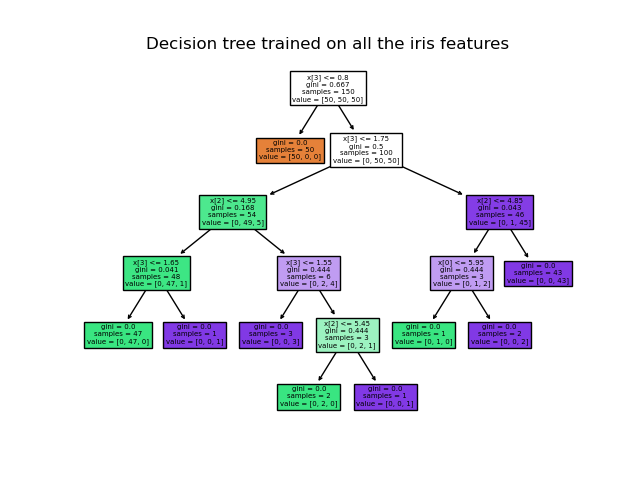
\includegraphics[width=0.75\textwidth]{image-3.png}
    \caption{Primer stabla odlučivanja obučena naspram Iris skupa podataka.}
\end{figure}

Takođe je uzeti u obzir smanjenje dimenzionalnosti (Principal component analysis - korišćen da vrši rastavljanje skupova podataka u skup rastućih ortogonalnih komponenti zarad pojašnjenja maksimalne količine disperzije\cite{pca}, Independent Component Analysis - rastavljanje višestrukih signala u sabirajuće podkomponente koje su maksimalno nezavisne\cite{ica}, Feature selection - radi se zarad pojačavanja tačnosti procenjivača ili ubrzavanja performansi\cite{fs}) zara boljeg nalaženja features-a koji su diskiriminativni.

\subsubsection{Multi-output problemi}
\label{sec:mop}
Problem nadgledanog učenja sa nekolicinom izlaza za predviđanje, gde je ciljana vrednost $Y$ u skupu podataka oblika 2D niza gde mu je broj redova jednak broju uzoraka, a broj kolona jedna broju izlaza za uzorak.
Ako nema međusobnih korelacija među izlazima, jednostavan način da se reši taj problem je pravljenje $n$ nezavisnih modela, tj. jedan model za svaki izlaz, i svaki nezavisno iskoristiti za predviđanje $n$ izlaza. Uočavajući da za iste ulaze izlazne vrednosti su međusobno srodne (u korelaciji), najbolje je sve $n$ izlaze istovremeno predvideti.
Pritom, tačnost generalizacije rezultujućeg procenjivača će obično se uvećati.

Zahtevaju se prateće promene naspram običnog binarnog stabla odlučivanja:
\begin{itemize}
    \item $n$ izlaznih vrednosti u listovima, umesto 1,
    \item Pri pravilu podele računati središnje umanjenje preko svih čitavih $n$ izlaza,
\end{itemize}

Klasifikaciju moguće demonstrirati kroz primer upotpunjivanja ljudskog lica sa multi-output estimators. Ulazi predstavljeni kroz vektor $X$ mogu biti pikseli gornjeg dela lica, a izlaz predstavljen vektorom $Y$ mogu biti pikseli donjeg dela lica, kao na slici 6.
\begin{figure}[h!]
    \centering
    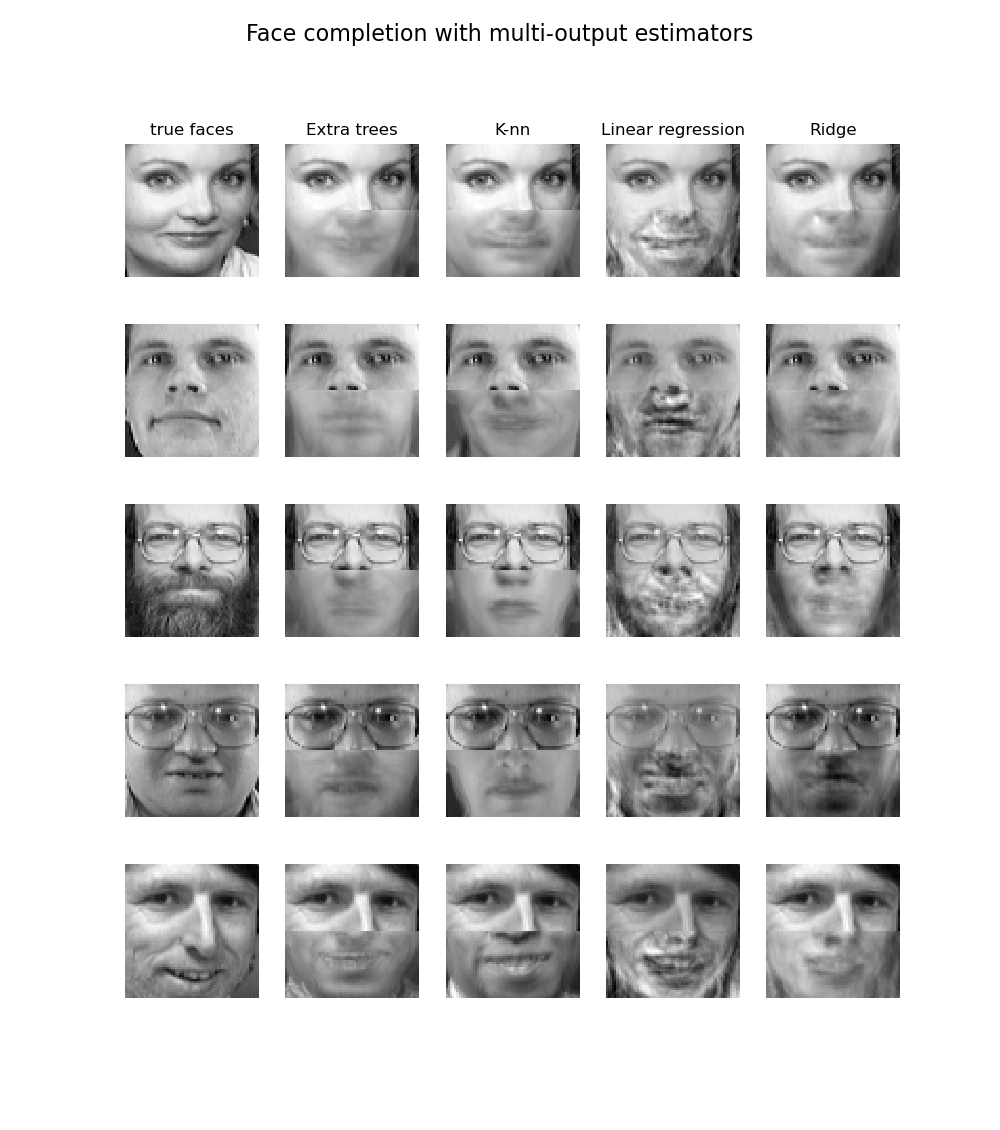
\includegraphics[width=0.5\textwidth]{image-4.png}
    \caption{Korišćen multi-output decision tree za prepoznavanje lica u drugoj koloni.}
\end{figure}

\subsubsection{Složenost izvršavanja}
Vremenska složenost da se izradi balansirano binarno stablo $O(n_{uzoraka}n_{features}\log(n_{uzoraka}))$, a pristupa je $O(\log(n_{uzoraka}))$.
Iako je cilj da stablo bude balansirano, ona neće biti nužno takva. Neka nagovestimo da podstabla su aprokisamtivno balansirajuća, cena svakog čvora uzima u obzir pretragu $O(n_{features})$ da bi se došlo do feature-a koji nudi najveću redukciju po \textit{kriterijumu nečistosti} gde mu je primer logaritamski gubitak (tj. information gain-u kojim dajemo značaj sagledanim obrascu u skupu podataka, kao i redukciji u entropiji: $Information Gain = entropija_\textit{čvora roditelja}-entropija_\textit{čvora deteta})$.\cite{entropy}
Cena $O(n_{features}n_{uzoraka}\log(n_{uzoraka}))$ za svaki čvor, vodeći se do ukupne cene naspram svih stabala (sumiranjem cena svakog od čvora) koja je $O(n_{features}n_{uzoraka}^{2}\log(n_{uzoraka}))$.

\subsubsection{Matematička formulacija}
Za čvor $m$, vektor obuke $x_i \in \mathbf{R}^n$, $i \in \{1,\dots,l\}$, vektor labele $y\in\mathbf{R}^l$. Podaci čvora $m$ su $Q_m$, sa $n_m$ uzorcima. Podela kandidat $\theta = (j, t_m)$, gde $j$ je feature, a $t_m$ prag. Podele skupa podataka su $Q_m^{left}(\theta)$ i $Q_m^{right}(\theta)$.
$$\begin{aligned}Q_m^{left}(\theta) = \{(x, y) | x_j \leq t_m\}\\Q_m^{right}(\theta) = Q_m \setminus Q_m^{left}(\theta)\end{aligned}$$

$H()$ je funkcija gubitka ili nečistosti i zavisi na osnovu oba tipa nadgledane obuke. 
$$G(Q_m, \theta) = \frac{n_m^{left}}{n_m} H(Q_m^{left}(\theta)) + \frac{n_m^{right}}{n_m} H(Q_m^{right}(\theta))$$

Vrši se odabir parametara zarad minimalizacije nečistosti:
$$\theta^* = \operatorname{argmin}_\theta  G(Q_m, \theta)$$

Slučaj rekurentne baze za podskupove $Q_m^{left}(\theta^*)$, $Q_m^{right}(\theta^*)$ dostizanje maksimalne dubine, $n_m < \min_{samples}$ ili $n_m = 1$.

\subsubsection{Kriterijum klasifikacije}
Se sagleda za čvor $m$, gde izlaz raspolaže vrednostima $0,\dots,K-1$.
$$p_{mk} = \frac{1}{n_m} \sum_{y \in Q_m} I(y = k)$$

Obavlja se računanje mera nečistosti:
\begin{itemize}
    \item Gini : $H(Q_m) = \sum_k p_{mk} (1 - p_{mk})$
    \item Log Loss ili entropija : $H(Q_m) = - \sum_k p_{mk} \log(p_{mk})$
\end{itemize}

Kriterijum entropije sračunat je uz pomoć Shannon entropije za dosupne klase. Sagleda verovatnoću predstavljenu kao učestalost zastupljenosti klasa uzoraka namenjenih za obuku koji su dosegli do nivoa lista stabla, lista $m$.
% Using the Shannon entropy as tree node splitting criterion is equivalent to minimizing the log loss (also known as cross-entropy and multinomial deviance) between the true labels
Kriterijum podele čvora stabla sprovodi se isto kao \textit{minimalizacija logaritmičkog gubitka}, tzv. \textit{cross-etropija}, \textit{multinomialna devijacija} mežu pravim labelama $y_i$ i probabilističkih predviđanja $T_k(x_i)$, modela stabla $T$ za klasu $k$. Računa se prvi odziv logaritmičkog gubitka za skup podataka $D$:

$$\mathrm{LL}(D, T) = -\frac{1}{n} \sum_{(x_i, y_i) \in D} \sum_k I(y_i = k) \log(T_k(x_i))$$

U klasifikatornom stablu, verovatnoće klasa predviđanja unutar čvorova listova su konstantni, gde $\forall (x_i, y_i) \in Q_m$, a sada je $T_k(x_i) = p_{mk}$, za svaku klasu $k$. Drugačiji zapis Shannon entropija za svaki list-čvor modela $T$, uzetim u obzir težinama naspram broja podataka obuke je: 
$$\mathrm{LL}(D, T) = \sum_{m \in T} \frac{n_m}{n} H(Q_m)$$


\subsubsection{Podrška po postojanosti nedostajućih vrednosti}
Za svaki potencijalni prag na neizgubljenim podacima, podela će se vršiti uz evaluaciju sa svim izgubljenim vrednostima uvrstavajući ih u levi ili desni čvor.
\\

Odluke će biti donošene na sledeći način:
\begin{itemize}
    \item Implicitno kada se vrši predviđanje uzorci sa izgubljenim vrednostima će biti klasifikovani sa klasama korišćenim u nailazećim podelama tokom treninga.
    \item Pri situaciji da kriterim evaluacije je isti za oba čvora, tada se u neizvesnosti eksplicitno uvrštava izgubljena vrednost na desnu stranu prilikom vršenja predviđanja. Podela je ustanovljena gde sve izgubljene vrednosti idu na stranu jedno čvora potomka, a ostale (neizgubljene) na drugu.
    \item Ako prilikom obuke ne bude izgubljenih vrednosti za dati feature, onda tokom predviđanja nedostajućih vrednosti se mapira u čvoru potomka sa više zastupljenih uzoraka.
\end{itemize}    


\subsubsection{Odsecanje minimalnom cenom složenosti}
Algoritam koji je korišćen za odsecanje stabla zarad izbegavanje situacije overfitting-a. a ima parametre:
\begin{itemize}
    \item $\alpha\ge0$ - parametar složenosti,
    \item $T$ - stablo,
    \item $R_\alpha(T)$ - cena složenosti.
    \item $|\widetilde{T}|$ - broj termalnih čvorova (listaova) u $T$
    \item $R(T)$ - tradicionalno ustanovljen kao ukupna stopa loše klasifikovanih termalnih čvorova (npr. ukupna nečistoća težina uzoraka termalnih čvorova - kao kriterijum)
\end{itemize}

$$R_\alpha(T) = R(T) + \alpha|\widetilde{T}|$$

Minimalna cena složenosti odecanja ustanovljena je u podstablu $T$ koji minimalizuje $R_\alpha(T)$. 
Cena složenosti kao mera jedinog čvora je $R_\alpha(t)=R(t)+\alpha$, za granu $T_t$ sagledanu kao stablo čvora korena $t$. Obično je nečistoća čvora veća od sume nečistoća termalnih čvorova $R(T_t)<R(t)$.

Određuje se efektivna vrednost $\alpha$ gde $R_\alpha(T_t)=R_\alpha(t)$ ili $\alpha_{eff}(t)=\frac{R(t)-R(T_t)}{|T|-1}$.


Netermalni čvorovi sa najmanjom vrednošću $\alpha_{eff}$ su veza koja treba biti odsečena.


Postupak se terminira kada je minimalna vrednost $\alpha_{eff}$ stabla koja je odsečena veća od unapred podešene $ccp_{alpha}$ vrednosti\cite{ccpalpha}.

\newpage

\subsection{Slučajne šume\cite{ensamblerf}}
Meta-procenjivač (metod ansambla) nad više klasifikatora slučajnih stabala nad raznolikim poduzorcima skupa podataka koji se koriste pri ustanovljavanju proseka tačnosti predviđanja (prikaz na slici 7.) i upravljanje overfitting-om.\cite{rf} Ističe se kao tehnika pomešati i kombinovati (preturb and combine; kreira više verzija datog grafa, primenjuje funkciju cena za čvorve pojedinačno za svaki graf, ukombinuje rezultate\cite{pnc}) namenjenog za stabla i sa time je uveden koncept nasumičnosti u konstrukcije klasifikacija. 

\begin{figure}[h!]
    \centering
    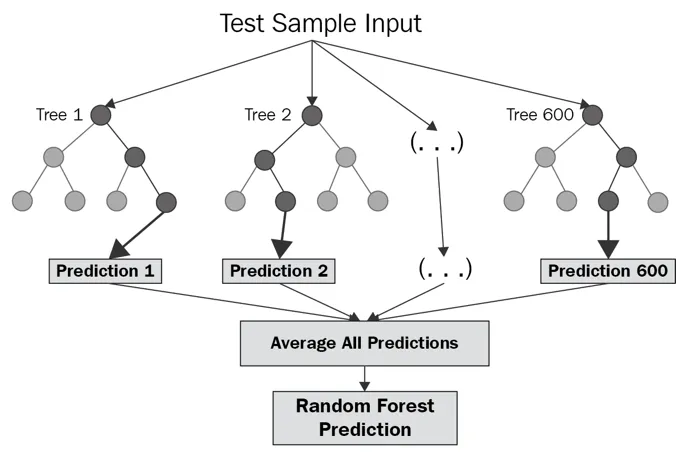
\includegraphics[width=0.5\textwidth]{image-6.png}
    \caption{Plan predviđanja slučajnih šuma.}
\end{figure}

Podržavaju proširenje na probleme više izlaza kao što je pomenuto u sekciji \hyperref[sec:mop]{2.2.1}.

Svako stablo u ansamblu građeno je iz uzorka sa zamenom (bootstrap uzorak) iz trening skupa.
Pri gradnji stabla podeli po svakom čvoru, najbolja podela je se pravi pri iscrpnoj pretrazi vrednosti features-a ili po nasumičnom skupu veličine naspram broja najviše mogućih features-a koja je unapred podešena. Cilj je izbeći visoku disperziju i overfitting procenjivača slučajnih šuma. Uvođenjem efekta nasumičnosti razložilo je greške pri predviđanju, a pri uzimanju proseka - neke greške su eliminisane. Zauzvrat, moguće je naići na blag porast cene u bias-u. 

Neki od kombinacije klasifikatora služe računanjem proseka, neki se koriste ``glasanjem'' za posebnu klasu.

\subsubsection{Unapred postavljeni parametri}
Glavni parametri zaslužni za prilagođavanje koji su korišćeni su \textit{broj procenjivača} i \textit{broj najviše features-a}, a može i da bude nekad \textit{broj stabala}. Preporuka je da budu veće vrednosti parametara, ističe se zahtevnost računa kao ishod. Nakon nekog kritičnog broja količine stabala ishoduje stagnaciji boljitka performansi. Sporedna veličina nasumičnih podskupova features-a se uzima u obzir kada se po čvoru vrši podela - što je niža to je veće umanjenje u disperziji, a veće pojačanje bias-a, sa manjom vrednošću je dosegnuta veća nasumičnost. Moguće je podesiti i \textit{najveću dubinu} i \textit{minimalan broj podela uzoraka}. Preporuka je da se izvrši cross-validation proces (ima moć da poredi i vrši odabir, manje se vezuje za određene koncepte nego druge tehnike predviđanja\cite{cv}) pri najbolje moguće podešenim parametrima. Moguće je podesiti zamenu uzorka (bootstrap mogućnost) gde greška generalizacije biva procenjena sa običnim uzorcima, uz bootstrap-bagging agregacije. 

Paralelizacija je moguća i ustanovljava paralelno izračunavanje predviđanja. Moguće je ekspilicitno podesiti broj zadataka koji će se izvršiti nad tom količinom jezgara u procesoru istovremeno. Vidljivo će biti uvećan performans pri radu sa većim brojem stabala ili pri radu sa većom količinom podataka na samom stablu.

Rangiranje srodnosti (npr. dubina) feature-a korišćeno je kada čvor odluke u stablu ustanovljava \textit{važnost feature-a} sve qdo predvidljivosti ciljane promenljive. Features-i korišćeni na vrhu stabla dprinose konačnom predviđanju krupnije frakcije ulaznih uzoraka. Očekivana frakcija uzoraka doprinosi pri proceni srodne važnosti features-a. U nekim sistemima frakcije uzoraka, kako feature doprinosi se uz kombinaciju umanjenja nečistosti po podeli pravi normalizovane procene za snagu predvđanja po feature-u. Po vršenju uprosečavanja procene moći predviđanja nad nekolicinom nasumičnih stabala se smanjuje disperzija takvih procena i njihovih korišćenja uz odabire feature-a - MDI (središnje opadanje u nečistosti).
Tim sračunavanjima feature važnosti zasnovanih na nečistosti sleduju 2 mane koje vode u zablude:
\begin{itemize}
    \item Sračunatim statistikama (funkcijom uzoraka; slučajnim promenljivama) svedenim iz trening skupa i sa time nas ne informiše o tome koji features-i su najvažniji da bi se napravile dobra predviđanja po priloženim skupovima podataka.
    \item Daje se prednost features-ima visokog kardinaliteta, pa i više jednoznačnih vrednosti. Permutacija važnosti feature-a (tehnika za obuku modela po statističkim performansama, korisna za nelinearne, neprovidne procenjivače koji uključuju nasumično pretumbavanje vrednosti posebnog feature-a i posmatranje degradacije rezultata ocene modela; ustanovljava se koliko se model osanja na određeni feature)\cite{permutation} je alternativa sračunavanjima feature važnosti zasnovanih na nečistosti, i eliminacija problema oslanjanja na feature, prikaz na slici 8. Dovodi se pojam \textit{važnosti permutacija} naspram MDI-a.
\end{itemize}
    \begin{figure}[h!]
        \centering
        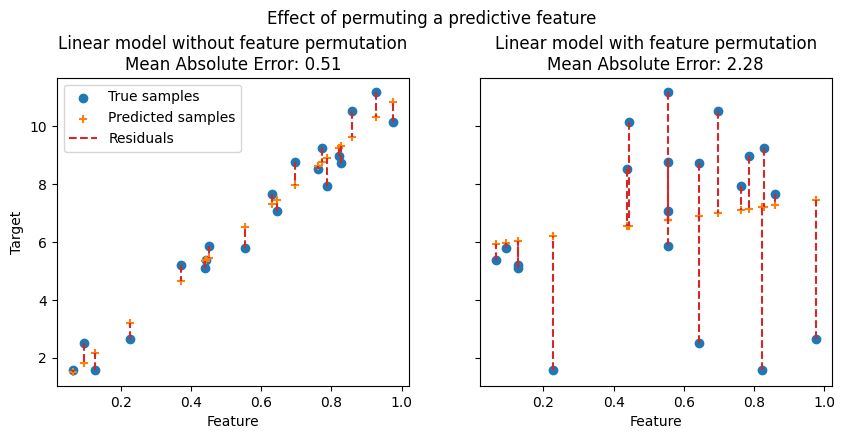
\includegraphics[width=0.5\textwidth]{image-9.png}
        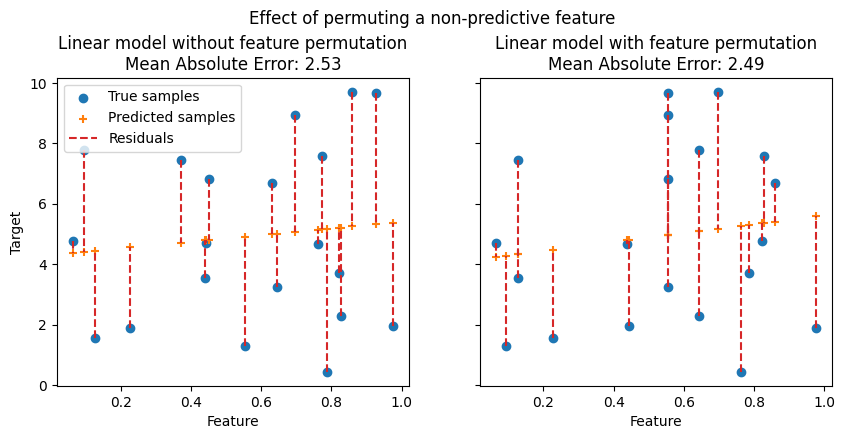
\includegraphics[width=0.5\textwidth]{image-7.png}
        \caption{Grafici sračunavanjima feature važnosti zasnovanih na nečistosti i permutacija važnosti feature-a (po kolonama) u okolnostima svojstva (ne)predvidljivog feature-a (po redovima).}
    \end{figure}
    
    Na slici 9. je dat primer korišćenja ekstremnih slučajnih šuma koji demonstriraju primenu feature važnosti po primeru individualnih piksela za svrhe prepoznavanje lica, što je svetlija tačka piksela to je važnost feature-a poklopljena pri funkcije procene predviđanja.
    \begin{figure}[h!]
        \centering
        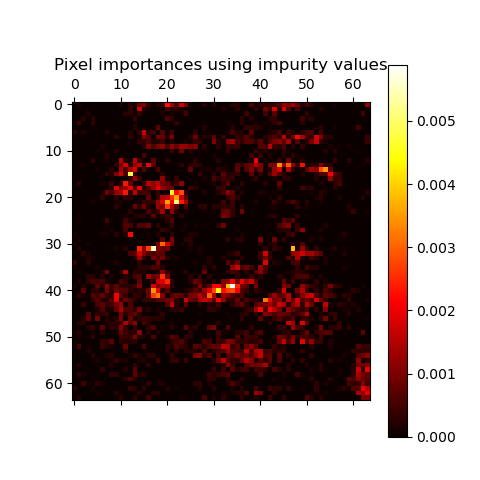
\includegraphics[width=0.32\textwidth]{image-8.png}
        \caption{Važnost piksela sa paralelnim slučajnim šumama, pri prepoznavanju lica.}
    \end{figure}

 
\newpage

\subsection{Klasifikacija naivnim Bajesom\cite{nb}}
Metode naivnog Bajesa se zasnimavju na primeni Bajesove teoreme sa "naivnim" pretpostavkama naspram nezavisnosti uslova među parovima features-a datih vrednosti klasa promenljivih.

\begin{figure}[h!]
    \centering
    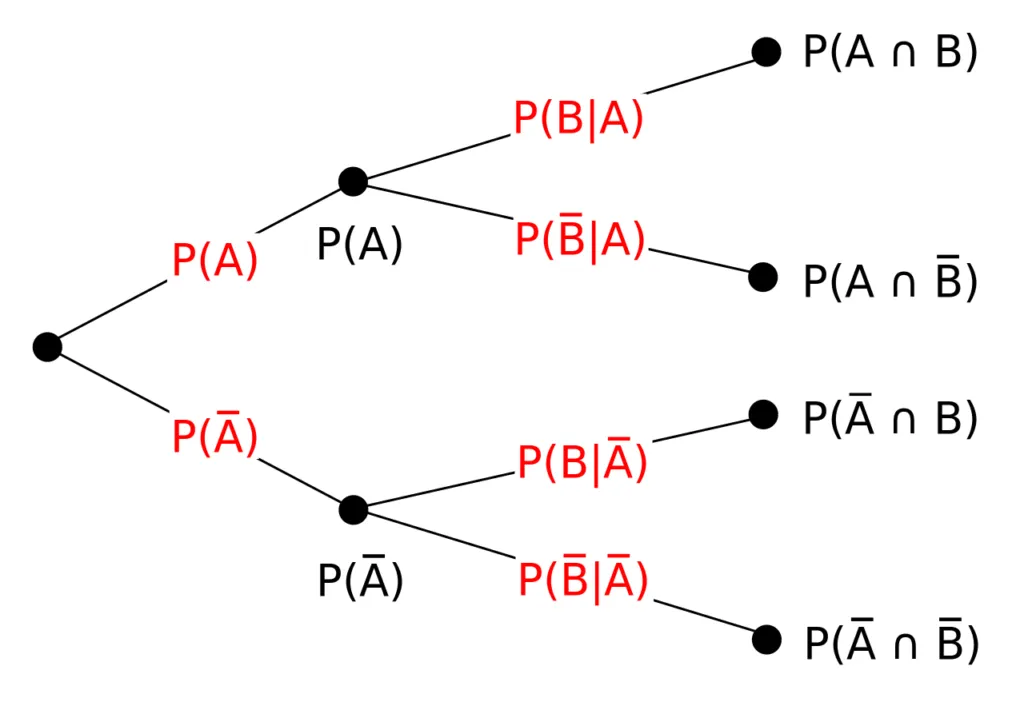
\includegraphics[width=0.3\textwidth]{image-10}
    \caption{\centering Dijagram stabla verovatnoća po nivoima događaja za formulu uslovne verovatnoće $P(A\cap B) = P(B|A)P(A)$, tj. $P(B|A) = \frac{P(A\cap B)}{P(A)} = \frac{P(A|B)P(B)}{P(A)}$.}
\end{figure}

 Bajesova teorema ustanovljava odnos promenljive $y$ (namenjena za vrednosti klasa uzoraka) i zavisnih $x_i$-eva (namenjena za feature vrednosti uzoraka; zavisnost delimično predstavljena slikom 10.), za $i=\overline{1,n}$:
$$P(y \mid x_1, \dots, x_n) = \frac{P(y) P(x_1, \dots, x_n \mid y)}
                                 {P(x_1, \dots, x_n)}$$

Gde je:
\begin{itemize}
    \item $P(y)$ - $prior$ verovatnoća ishoda da se događaj nailaženja vrednosti klase $y$ desi pri predviđanju,
    \item $P(x_1, \dots, x_n)$ - verovatnoća da se desi nailaženje nove posebne torke vrednosti features-a uzorka pri predviđanju, tj. ovde predstavljenih u vidu niza promenljivih, tzv. \textit{pokrića (evidence)},
    \item $P(x_1, \dots, x_n \mid y)$ - verovatnoća \textit{verodostojnosti (likelihood)},
    \item $P(y \mid x_1, \dots, x_n)$ - \textit{posterior verovatnoća}. Po kombinovanju sagledane informacije, ažurira se a priori informacija po sagledanju klase $y$.\cite{nb-names}
\end{itemize}

$$posterior = \frac{prior \times likelihood}{{evidence}}$$

\vbox{}
Verovatnoća \textit{nezavisnosti događaja}\cite{probabiliy-independence} je $P(A|B)=P(A)$ (tj. $P(A \cap B)=P(A)P(B)$; npr. računanje verovatnoće tokom bacanja 2 novčića - koji su međusobno \textbf{zavisna 2 događaja}, i nakon toga, biranje ta dva). 

I definiciji da je \textit{uslovna nezavisnost} ustanovljena događajem $C$, gde $P(C) > 0$ ako 
$$P(A \cap B|C)=P(A|C)P(B|C).$$
Pritom, koristeći se $P(A|B)=\frac{P(A \cap B)}{P(B)}$, ako $P(B) > 0$. I ako je $P(B|C), P(C)\ne 0$ onda svedemo na:
$$P(A|B\cap C)=\frac{P(A \cap B|C)}{P(B|C)}.$$
To uradimo postupkom: $P(A|B\cap C)= \frac{P(A\cap B\cap C)}{P(B\cap C)} = \frac{P(A \cap B|C)\cancel{P(C)}}{P(B|C)\cancel{P(C)}} =\frac{P(A \cap B|C)}{P(B|C)}$

\newpage

Nakon toga, ako su $A$ i $B$ uslovno nezavisne od $C$.
$$\begin{aligned}
    P(A|B\cap C) &=\frac{P(A \cap B|C)}{P(B|C)} \\
    &=\frac{P(A|C)P(B|C)}{P(B|C)}
    &=P(A|C).
\end{aligned}
$$
Ako $A$ i $B$ su uslovno nezavisni ustanovljenim $C$, tada važi da:
$$P(A | B,C)=P(A|C).$$

Koristeći se ovime kao naivnom uslovnim nezavisnim predviđanjem da:
$$P(x_i | y, x_1, \dots, x_{i-1}, x_{i+1}, \dots, x_n) = P(x_i | y)$$
Potom, $\forall i$ odnos je pojednostavljen (uz svojstvo nezavisnosti događaja formulom $P(A \cap B)=P(A)P(B)$) na:
$$P(y \mid x_1, \dots, x_n) = \frac{P(y) \prod_{i=1}^{n} P(x_i \mid y)}
{P(x_1, \dots, x_n)}$$
Uzimajući u obzir da je $P(x_1, \dots, x_n)$ konstantno pošto važi za ulaz (features-i), radi se klasifikaciono pravilo za neko $k$:
$$\begin{aligned}P(y \mid x_1, \dots, x_n) = k* P(y) \prod_{i=1}^{n} P(x_i \mid y)\\\Downarrow\\\hat{y} = \arg\max_y P(y) \prod_{i=1}^{n} P(x_i \mid y),\end{aligned}$$
gde se koristi procena $\hat{y}$ - \textit{maksimalne a posteriori} - MAP za izvođenje $P(y)$ i $P(x_i|z)$. Prethodni iskaz pre dobijenog MAP-a je srodan po učestalosti klase $y$  koja se nalazi u trening skupu.

\vbox{}
\textbf{Naivni Bajes klasifikatori se razlikuju najglavnije po predviđanjima koje vrše za distribuciju $P(x_i \mid y)$.}

Uprkos preuprošćenim predviđanjima, naivni Bajes klasifikatori rade vrlo pouzdano u realnom svetu, u slučaju klasifikacije dokumenata i filtriranja spamova. Ne zahtevaju krupne skupove podataka zarad obuke da bi procenjivali po neophodnim parametrima. Obučavači naivnog Bajesa i klasifikatori mogu biti ekstremno brzi u poređenju sa više sofisticiranijim metodama. Raskopčavanjem (rasparivanje, decoupling) klasa uslovljenog feature-a se raspodeljuje (distribuira) ponaosob vršeći procenu nezavisno po dimenzionoj distribuciji. Ovim se olakšava pitanje dimenzionalnosti. Zauzgred, iako je poznat kao pouzdan klasifikator, poznat je i kao loš procenjivač, pa verovatnoće na izlaza ne uzimati ``zdravo za gotovo''.

Neke od vrsta klasifikatora naivnog Bajesa su:
\begin{itemize}
    \item \textit{Gausov naivni Bajes} - likelihood features-a ustanovljeni kao Gausijanski (distribucija verovatnoća koja je simetrična naspram očekivane vrednosti - središta, prikazivanje da neki od podataka su frekventniji po zastupljenosti od ostalih, više od središnje vrednosti)\cite{gaus}, gde su $\sigma_y = \sqrt{\frac{\sum_{i=1}^n(x-\mu_y)^2}{n-1}}$ (standardna devijacija za promenljivu klase) i $\mu_y = {1\over n} \sum_{i=1}^n x_i $ (očekivanje/središnja vrednost za promenljivu klase) procenjeni putem maksimalnog likelihood-a.
    $$P(x_i \mid y) = \frac{1}{\sqrt{2\pi\sigma^2_y}} e^{-\frac{(x_i - \mu_y)^2}{2\sigma^2_y}}$$
    \begin{figure}[h!]
        \centering
        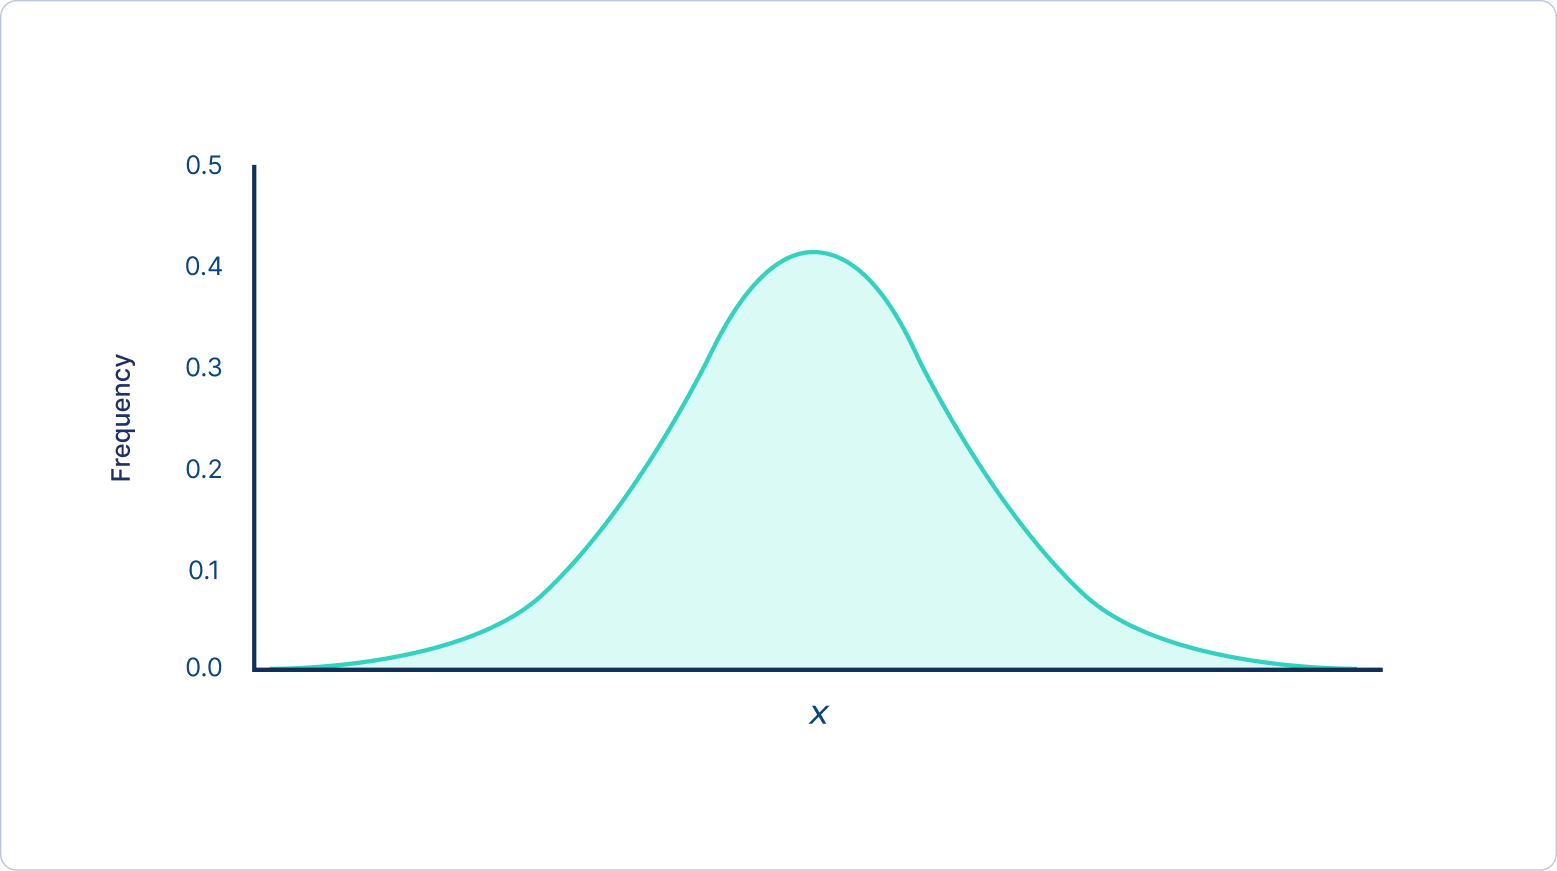
\includegraphics[width=0.5\textwidth]{image-11.png}
        \caption{\centering Gausova Bell kriva distribucije, učestalost zastupljenosti po vrednosti.}
    \end{figure}
    \item \textit{Multinomijalni naivni Bajes} - namenjen za multinomijalno distribuirane (generalizacija binomne distribucije koja diskretno obrađuje do ishoda 2 ili više vrednosti fiksnih verovatnoća za svaku vrednost nezavisno generisanih\cite{multinomial}) podatke, jedan od uobičajenih Bajesovih vrsta namenjenih za tekstualnu klasifikaciju (podaci su tipično reprezentacija brojčani vektori reči, vizuelizovan rezultat na slici 12., iako tf-idf vektori kao alternativa su poznati kao pouzdani u praksi koji mogu biti razgranati na 2 slučaja učestalost pojma - TF i inverzne učestalosti dokumenta - IDF).
    
    \begin{figure}[h!]
        \centering
        
\includegraphics[width=0.5\textwidth]{image-12.png}
        \caption{\centering Multinomijalni naivni Bajes model daje ovakav rezultat naknadno vizuelizovan, ključna reč veća po svojoj učestalosti.}
    \end{figure}
    
    Distribucija je parametrizovana po vektorima $\theta_y = (\theta_{y1},\dots,\theta_{yn})$ $\forall y$ gde je $n$ broj features-a (u tekst klasifikaciji, veličina rečnika) i $\theta_{yi} = P(x_i \mid y)$ kao verovatnoća feature-a i koji se pojavljuje u uzorcima udeljenim klasi y.
    
    Parametri $\theta_y$ su procenjeni po \textit{smooth-ovanoj (uglađenoj)} veziji maksimalne verodostojnosti (likelihood-a), tj. brojke relativne učestalosti: 

    $$\hat{\theta}_{yi} = \frac{ N_{yi} + \alpha}{N_y + \alpha n}$$

    gde $N_{yi} = \sum_{x \in T} x_i$ je broj puta gde feature $i$ nailazi pri klasi $y$ u trening skupu $T$, a $N_y = \sum_{i=1}^n N_{yi}$ je ukupno prebrajanje svih features-a za klasu $y$.

    Smoothing zastupljen uz $\alpha\ge 0$ odgovoran za features-e neuvrštene među uzorke obuke i eliminiše nepogodnosti u vezi verovatnoća jednakih 0 u daljim sračunavanjima. Podešavanjem $\alpha = 1$ dobija se \textit{Laplace smoothing}, dok uz $\alpha < 1$ dobija se \textit{Lidstone smoothing}.

    \item \textit{Komplementarni naivni Bajes (CNB)} - proširenje standardnog algoritma multinomialnog naivnog Bajesa - MNB koji je posebno namenjen za nebalansirane skupove podataka. CNB koristi statistiku komplementa svake posebno klase zarad izračunavanja težina modela. Od konstruktora ovog algoritma je izjavljeno da su proračuni parametara empirički više pouzdanija nego kod MNB-a. CNB često prevazilazi MNB (do uočljivih razmera) pri zadacima klasfikacija teksta.
    Postupak za sračunavanje težina sledi:
    $$ \begin{aligned}\hat{\theta}_{ci} = \frac{\alpha_i + \sum_{j:y_j \neq c} d_{ij}}
        {\alpha + \sum_{j:y_j \neq c} \sum_{k} d_{kj}}\\w_{ci} = \log \hat{\theta}_{ci}\\w_{ci} = \frac{w_{ci}}{\sum_{j} |w_{cj}|}\end{aligned}$$
    gde sumiranja svih dokumenata $j$ nisu u klasi $c$, $d_{ij}$ je ili-ili brojka tf-idf vrednosti pojmova $i$ u dokumentu $j$, a $\alpha_i$ je smoothing hiperparametar kao kod MNB-a i $\alpha = \sum_i \alpha_i$. Druga normalizacija adresira težnju da duži dokumenti imaju zastupljeniji proračun parametra u MNB. Pravilo klasifikacije je: 
    $$\hat{c} = \arg\min_c \sum_{i} t_i w_{ci}$$
    tj. dokument dodeljen klasi je onaj sa \textit{najsiromašnijim} poklapljanjem komplementa.
    \item \textit{Bernulijev naivni Bajes (BNB)} - rade nad podacima distribuiranih na odgovornost višestruke Bernulijeve distribucije (slična geometrijskoj raspodeli, ali nisu iste)\cite{bernoulli}; tj. mogu biti više features-a, ali svaki ponaosob je predviđan da bude binarno-vrednovana (Bernilijeva, Bulova) promenljiva. Klasa zahteva uzorke da budu predstavljeni kao binarno-vrednovani feature vektori.
    Pravilo odluka za Bernilijev naivni Bajes zasnovan je na:
    
    $$P(x_i \mid y) = P(x_i = 1 \mid y) x_i + (1 - P(x_i = 1 \mid y)) (1 - x_i)$$
    
    gde se razlikuje od MNB-ovog pravila po tome što ova eksplicitno kažnjava neispoljavanje feature-a $i$ koji jej indikator klase y, gde multinomijalna varijanta tome ne daje značaj prosto.

    U slučaju klasifikacije teksta, vektori pojavljivanja reči (pre nego vektori brojnosti reči) moguse koristiti pri obuci i korišćenju klasifikatora. Pogodniji za korišćenje kod kraćih dokumenata.

    \item \textit{Kategorički naivni Bajes} - zasnovan na podacima koji su kategorički distribuirani. Predviđaju da svaki feature posebno, opisan indeksom $i$ ima sopstvenu kategoričku distribuciju.
    Svaki feature $i$ je u trening skupu $X$ pretpostavljen klasi $y$. Skup indeksa uzoraka je definisan $J = \{1,\dots,m\}$, gde m označava broj uzoraka.

    Verovatnoća kategorije $t$ u feature-u $i$ date klase c je procenjena kao:
    $$P(x_i = t \mid y = c \: ;\, \alpha) = \frac{ N_{tic} + \alpha}{N_{c} +
                                       \alpha n_i},$$
    gde $N_{tic} = |\{j \in J \mid x_{ij} = t, y_j = c\}|$ je broj puta kategorija $t$ se ispoljava u uzorcima $x_i$, koja pripada klasi $c$, dok $N_{c} = |\{ j \in J\mid y_j = c\}|$ je broj uzoraka sa klasama $c$, $\alpha$ je smoothing parametar i $n_i$ je broj dostupnih kategorija u feature-u $i$.

    Obično se $X$ enkodira po ordinalnom enkoderu\cite{ordinal} u praksi kategroije reprezentovane za svaki feature $i$ brojevima $\overline{0,n_i-1}$ gde je $n_i$ broj dostupnih kategorija feature-a $i$.
\end{itemize}

Naivni Bajes modeli mogu da se susretnu sa problemima klasifikacija visokih razmera u slučaju pun trening skup ne može se smestiti u memoriju. Neki od sistema koriste metode koji klasifikatori inkrementalno vrše klasifikacije, tj. \textit{out-of-core (izvan srži)} klasifikacije. Može da vrši iscrpne proračune sa time je opet preporučljiv isparčan rad (da bi se izbeglo preopterećenje primarne memorije) i pri ovom rešenju.
\newpage

\subsection{Mašina potpornih vektora (SVM)\cite{svm}}

Korišćeni za klasifikacije, regresije i detekciju outliers-a (diskrimnatornih uzoraka u odnosu na druge). Kasnije će detaljnije osnovna metodologija biti predstavljena, a sada idu pojašnjenja za osobine SVM-a.

Ne pružaju direktno procene verovatnoća, sračunati su iscrpnim 5-fold cross-validacijama (uzorke izdeli u 5 grupa, tzv. folds-e, koristeći se ``ostavi 1 van'' strategijom, obuka zarad predviđanja se radi nad 5-1=4 folds-a, a onaj 1 fold je ostavljen za testiranje, prikazani na slici 14.)\cite{cv}.

\begin{figure}[h!]
    \centering
    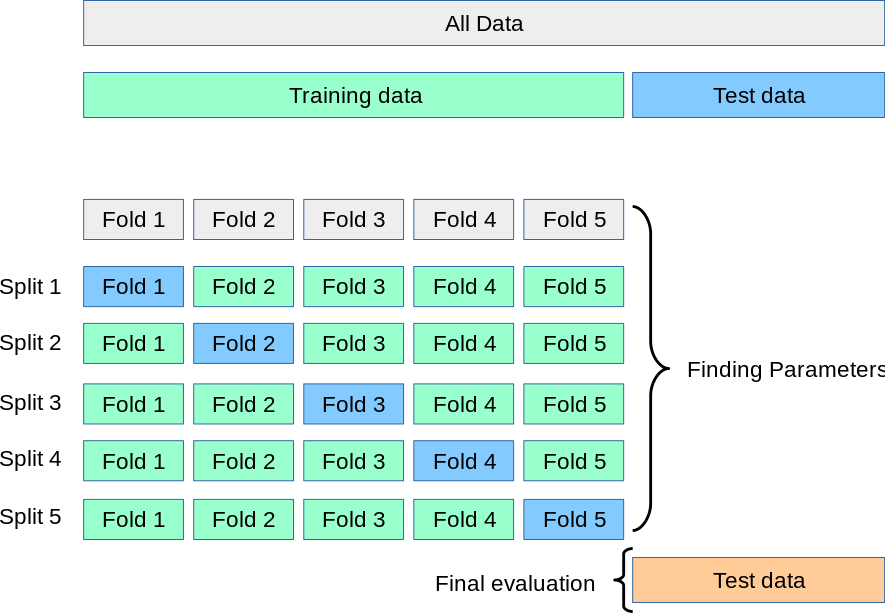
\includegraphics[width=0.5\textwidth]{image-20.png}
    \caption{\centering primer 5-fold cross-validacije i naknadnog testiranja posle predviđanja crossvalidaion-om}
\end{figure}

Neki razvijeni sistemi SVM-a podržavaju \textit{guste} i \textit{raspršene} uzoračke vektore kao ulaze. 
Klasifikacije koje se obavljaju mogu biti binarne i multiklasifikatorne za skup podataka.

\begin{figure}[h!]
    \centering
    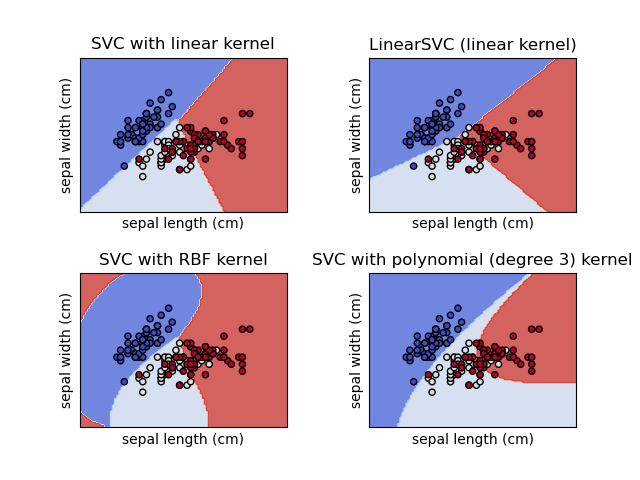
\includegraphics[width=0.75\textwidth]{image-13.png}
    \caption{2 feature-a iris skupa podataka upoređena po različitim režimima}
\end{figure}

\textit{Nu-SVM klasifikatori} su malo specifičniji i imaju različite matematičke formulacije. \textit{Linearni-SVM klasifikatori} su brža verzija SVM klasifikatora u slučaju linearnih kernela, koristi gubitke \textit{kvadratnih hindževa} (alternativa cross-entropiji - ustanovljava greške kada su znakovi prisutni među tačnim i predviđenim vrednostima i u ovom slučaju taj sračunat gubitak se kvadrira)\cite{hinge}, isto reguliše preseke pri radu sa LIBLINEAR rešavačima\cite{liblinear}, ako su postavljeni kao potrebni. Moguće je vršiti postupak \textit{skaliranja presecanja} (sintetički feature - veštački izgenerisan / nije na osnovu događaja iz realnog sveta - sa konstantnom vrednošću jednaka je ovoj meri, pa je primenjena na vektor uzorka i sagledana je kao multiplikacija težine sintetičkog feature-a)\cite{intercept-scaling}\cite{syntetic-feature} kao vid \textit{finetunning-a} (finog podešavanja) zarad eliminisanja efekta gubitka, ovo omogućava po principu presecanja da se ispoljavaju različiti ishodi regularizacija naspram drugih features-a. Klasifikacije linearnih SVM klasifikatora rezultuju drugačijim ocenama od ostala dva SVM klasifikatora.

Tu su, takođe, dostupni primeri \textit{nelinearnih SVM-ova} (koji koriste RBF kernele - kasnije će se pominjati zarad rešavanja problema linearne neseparabilnosti, prikaz na slici 16.)\cite{nonlinsvm}, \textit{SVM-Anova}(rad sa šumovima od uzoraka pri klasifikaciji)\cite{anova}.

\begin{figure}[h!]
    \centering
    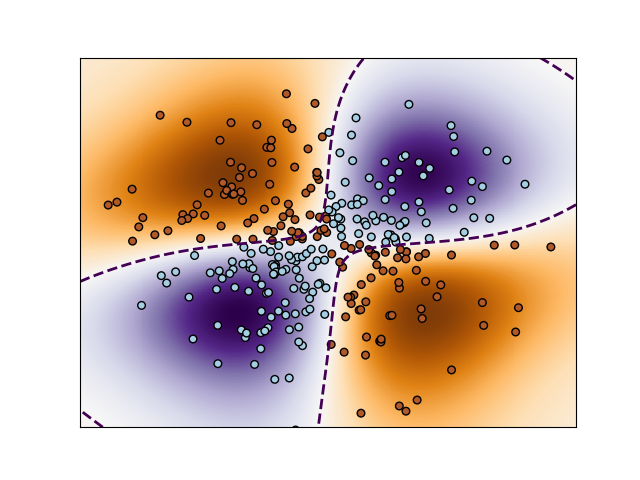
\includegraphics[width=0.5\textwidth]{image-14.png}
    \caption{Primer funkcije odlučivanja obučene nelinearnim SVM-om}
\end{figure}





Pri nebalansiranim problemima, gde je poželjno dati više važnosti određenim klasama ili određenim posebnim uzorcima, tu se dodeljuje težinski faktor.
SVM klasifikator sa sobom može da nosi težinski faktor klase pri metodi obuke uz multiplikaciju parametra kažnjavanja, slika 17. predstavlja granicu odlučivanja za nebalansirajući problem sa i bez uticaja težinskog faktora.  

\begin{figure}[h!]
    \centering
    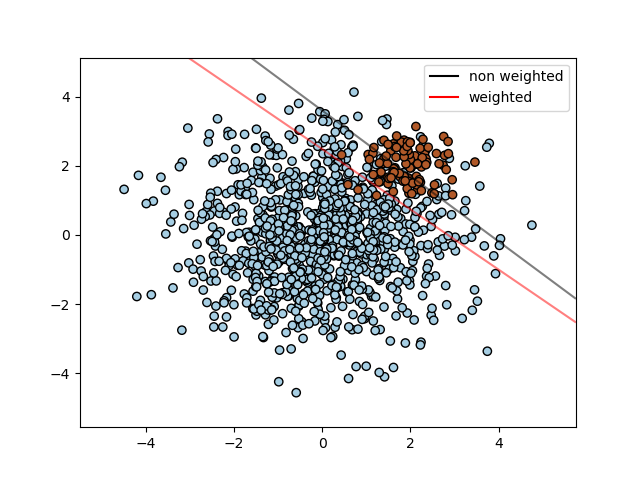
\includegraphics[width=0.5\textwidth]{image-15.png}
    \caption{Granice odlučivanja pri nebalansiranom problemu uz/bez težinskog faktora klase}
\end{figure}

SVM, nuSVM, linearni SVM klasifikatori (prikazani na na slici 15.), jednoklasni SVM metoda (zaslužna za outlier detekcije) koriste pri obuci težinski faktor uzoraka. Ohrabriće se klasifikator težinskim faktorom uz multipliciranje nekim parametrom pozitivne decimalne vrednosti kažnjavanja  da vrši prave klasifikacije nad uzorcima. Prikaz na slici 18. je efekat težinskog faktora uzoraka po granici odlučivanja.

\begin{figure}[h!]
    \centering
    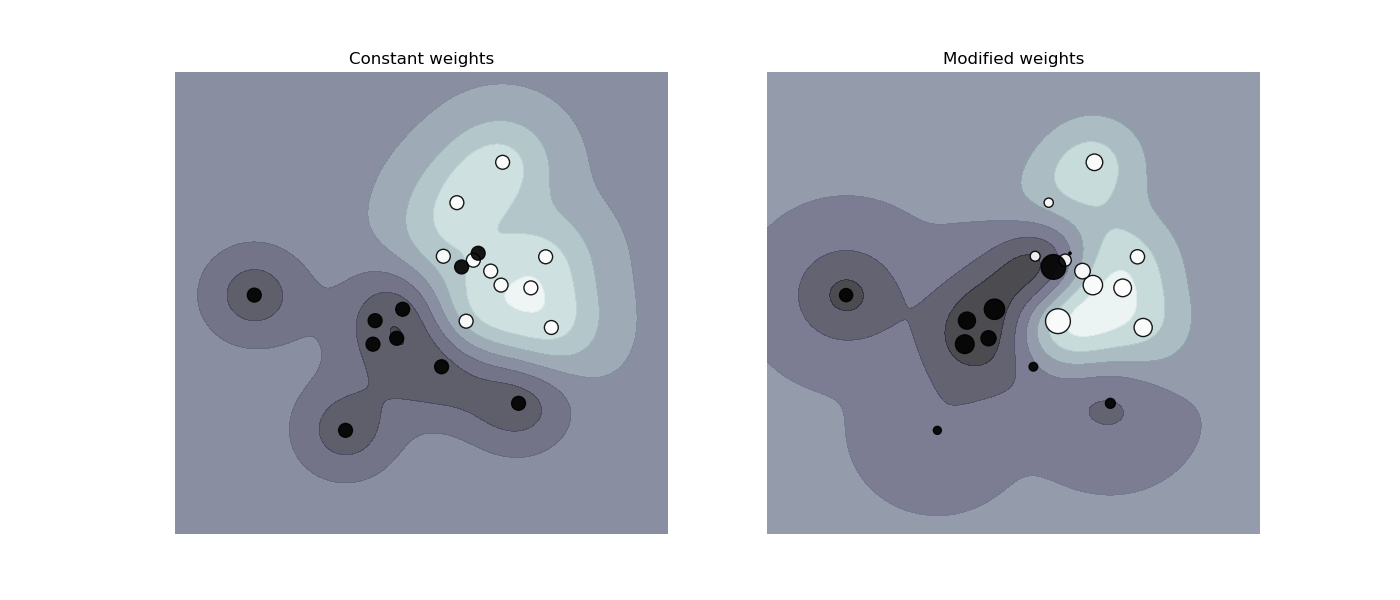
\includegraphics[width=0.75\textwidth]{image-16.png}
    \caption{Granice odlučivanja pri nebalansiranom problemu bez/uz težinski faktor uzoraka}
\end{figure}

SVM su snažni alati, ali zahtevnosti sračunavanja i skladišta rapidno se uvećavaju po broju vektora obuke. Srž SVM-a je \textit{kvadratni programerski problem (QP - namenjen za rad od bilinearnih do (ne)jednačinama polinoma 2. stepena, korišćen za obradu slika i signala)}\cite{qp}, izdvajajući potporne vektore od ostalih trening podataka. QP rešavač može se skalirati u granicama $O(n_{features} \times {n_{uzoraka}}^2)$ prema $O(n_{features} \times n_{uzoraka}^3)$, ako su podaci vrlo raspršeni $n_{uzoraka}$ bi trebalo biti zamenjeni sa \textit{prosečnim brojem nenula features-a u vektoru uzoraka}.

Za linearne slučajeve korišćen je linearni SVM klasifikator uz LIBLINEAR rešavač koji je pogodan da se skalira skoro linearno na milione uzoraka i/ili features-a. 

U praktičnom smislu preproučuje se da se izbegavaju kopije podataka pri radu sa linearnim klasifikatorima, oprez sa veličinom cache memorije pri odabiru kernela, sagledanje parametra za rad sa težinskim faktorima u slučaju da su šumoviti uzorci u skupu podataka (vremenska složenost može biti uvećana u suprotnom), da se skaliraju prodaci koriščenjem pipeline-a\cite{pipeline} - predviđenog za sekvencijalno transformisanje i obradu podataka kroz sve do konačnog predviđača, sagledanje parametra sužavanaja za umanjenje vremena udeljenog obuci, parametar aproksimiranja grešaka pri obuci, usaglašavanja parametra kažnjavanja sa ne(balansiranosti) podataka, podešavanja nasumičnosti, podešavanja L1 kažnjavanja linearnom SVM klasfikatoru.

\vbox{}
\textbf{Kernel funkcije} koje su dostupne su:
\begin{itemize}
    \item linearni : $\langle x, x'\rangle$ - skalarni proizvod vektora između tačaka uzoraka,
    \item polinomijalan : $(\gamma \langle x, x'\rangle + r)^d$, stepena $d$ i posebnog koeficijenta $r$,
    \item RBF : $\exp(-\gamma \|x-x'\|^2)$ - predstavljen parametrom $\gamma>0$,
    \item sigmoidna : $\tanh(\gamma \langle x,x'\rangle + r)$.
\end{itemize}

\vbox{}
Radial Basis-a funkcije - RBF kernel ima 2 parametra koji su sagledani\cite{rbfparams}:

\begin{itemize}
    \item $C$ - raspolaže izbegavanjem obukom uzorcima loše klasifikacije u odnosu na površ odlučivanja za sve SVM kernele; uspostavlja glatkost površi odlučivanja; visoka vrednost je namenjena za sve uzorke da obuka bude neprikosnovena) i 
    \item $\gamma$ - ustanovljava koliko ima uticaja jedan uzorak pri obuci. Višom vrednošću uzorci moraju biti bliži međusobno da bi bili prikladni.
\end{itemize}
Preporučuje se rad sa hiperparametrima za nalaženje pogodnih vrednosti parametara.
Neki sistemi omogućuju definiciju prerađenih kernela. Moguće je za kernele koristiti Gram matricu $G$ (za skup $V$ od $m$ vektora elemenata iz $\mathbb{R}^n$ ona sadrži skalarne proizvode među vektorima iz $V$, tj. $g_{i,j} = v_i^Tv_j$; očuvava dužine izometrijom nakon transformacija)\cite{gram}\cite{isometry}.

\subsection{Metodologija}
SVM grade hiper-ravan ili skup hiper-ravni u visoko ili beskonačno dimenzionalnim prostorima. Intuitivno, dobra separacija je postignuta kada za hiper-ravan po najvećoj distanci bliskoj uzorcima bilo koje klase, tzv. \textit{funkcionalnoj margini}. Uopšteno, većom marginom dobija se niža generalizacija greškom klasifikatora. Slika 19. daje prikaz linearno separabilnog probleima 3 tačke predstavljaju uzorke na granicama margine, tzv. \textit{potpornim vektorima}.

\begin{figure}[h!]
    \centering
    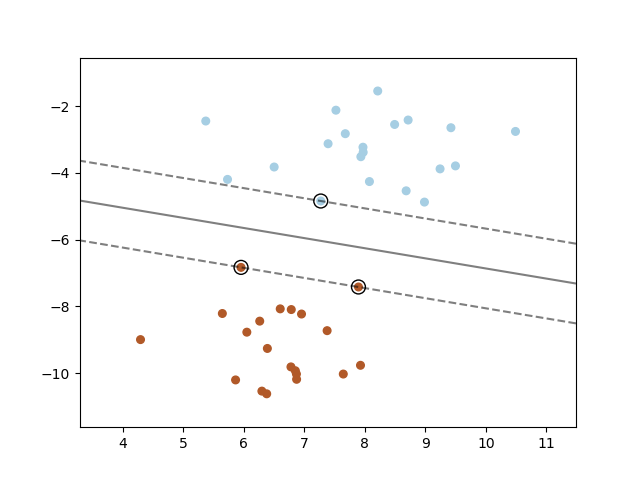
\includegraphics[width=0.5\textwidth]{image-17.png}
    \caption{Granice margine, potrporni vektori nad vizuelizacijom skupa podataka}
\end{figure}

Kada problem je linearno \textbf{neseparabilan} onda se uzorci nalaze u granici margina kao potporni vektori.

Datim vektorima obuke $x_i \in \mathbf{R}^p, i=\overline{1,n}$, u 2 klase vrednosti vektora $y \in \{-1, 1\}^n$, cilj je naći $w \in \mathbf{R}^p$ i naći $b\in \mathbf{R}^n$ tako da predviđanje je dato po $\text{sign} (w^T\phi(x) + b)$ je tačan za većinu uzoraka.

SVM klasifikacija rešava \textbf{glavni problem}:
$$\begin{aligned}\begin{aligned}
    \min_ {w, b, \zeta} \frac{1}{2} w^T w + C \sum_{i=1}^{n} \zeta_i \\
    \begin{aligned}
        \iff & y_i (w^T \phi (x_i) + b) \geq 1 - \zeta_i, \\
                              & \zeta_i \geq 0, i=1, ..., n
    \end{aligned}
\end{aligned}\end{aligned}$$
Intuitivno, poželjno je maksimizovati margine (minimizacijom $||w||^2 = w^Tw$), pritom nezgodno kažnjavanje se dešava pri netačnoj klasfikaciji uzorka ili pri upadanju granicu margina. Idealan slučaj je da važi $y_i (w^T \phi (x_i) + b) \ge 1$ za sve uzorke, ukazuje na perfektnu predikciju. Problemi nisu uvek savršeno separabilni sa hiper-ravnima, pa dopuštamo nekim uzorcima da budu na distanci $\zeta_i$ naspram njihove tačne granice margine. Kazneni parametar $C$ upravlja jačinom kazne i kao rezultat, deluje kao \textbf{parametar} inverzne \textbf{regularizacije}.

Sporedni problem naspram glavnog je:
$$
\begin{aligned}\begin{aligned}\min_{\alpha} \frac{1}{2} \alpha^T Q \alpha - e^T \alpha\\\begin{aligned}
    \iff & y^T \alpha = 0\\
    & 0 \leq \alpha_i \leq C, i=1, ..., n\end{aligned}\end{aligned}\end{aligned}
$$
gde $e = \begin{bmatrix}1 \\ 1 \\ \vdots \\ 1\end{bmatrix}$, i $Q$ je polu-definitna matrica (ako su joj sve jedinične vrednosti nenegativne, vršenim normiranjem)\cite{definitemx}. $Q_{ij} \equiv y_i y_j K(x_i, x_j)$, gde $K(x_i, x_j) = \phi (x_i)^T \phi (x_j)$ je \textbf{kernel}. \textit{Dualni koeficijenati} su $\alpha_i$, gde $\alpha \le sup((-\infty, C))$, i ona ispoljava činjenicu da vektori obuke su implicitno mapirani na (možda beskonačne) dimenzionalne prostore po funkciji $\phi$, tj. \textbf{kernel trik} (prikazan na slici 20.).

\begin{figure}[h!]
    \centering
    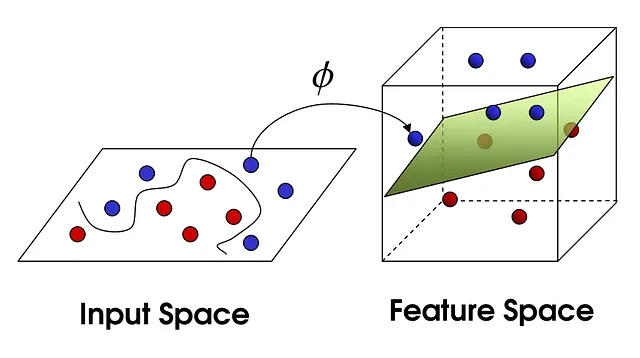
\includegraphics[width=0.5\textwidth]{image-18.png}
    \caption{Kernel trik}
\end{figure}

Čim je problem optimizacije razrešen, izlaz \textbf{funkcije odlučivanja} za dati uzorak biće:
$$\sum_{i\in SV} y_i \alpha_i K(x_i, x) + b$$
i predviđena klasa predodređena je njenim znakom. Moramo samo sumirati potporne vektore (tj. uzorke koji leže na margini) pošto \textbf{dualni koeficijenti su za ostale uzorke $\alpha_i = 0$}.

\vbox{}
Pojedini optimizatori $C$ parametar kažnjivanja označavaju sa $alpha$. Tačna jednakost količine regularizacije 2 modela zavisi od tačne funkcije cilja optimizacirane, gde za model u nekim primerima je $C = \frac{1}{alpha}$.

\vbox{}

\textbf{Linearni SVM klasifikator ima za svoj oblik svoj  glavni problem za rešavanje:}
$$\min_ {w, b} \frac{1}{2} w^T w + C \sum_{i=1}^{n}\max(0, 1 - y_i (w^T \phi(x_i) + b)),$$
važno je da se postavi primena hindža\cite{hinge}. Forma je direktno optimizovana po linearnoj SVM klasfikaciji, ali za razliku od dualne forme, ova ne uključuje skalarne proizvode među uzorcima, pritom kernel trik nije doveden u obzir. Ovo je bio razlog zašto linearni kernel je jedino podržan od ovog klasfiikatora ($\phi$ je funkcija idenititeta).

\vbox{}


\newpage
\subsection{K-najbližih suseda (kNN)\cite{knn}}

Ustupaju funkcionalnost za metode (ne)nadgledane obuke zasnovane na susedima. Nadgledano obučavanje zasnovano na susedima ima dve vrste, od kojih je klasifikaciju za podatke diskretnih labela, a drugi regresija. Princip iza metoda najbližih suseda (NN) je naći predefinisan broj najbližih trening uzoraka u odstojanju od tačke novog uzorka, pa tako predvide labelu iz trening uzoraka. Broj uzoraka može biti ili korisnički definisana konstanta $k$ (\textit{kNN}), ili samo da varira po gustini lokalnih tačaka (\textit{NN zasnovane po radiusu korisnički definisanog $r$}), prikazane na slici 21. 

\begin{figure}[h!]
    \centering
    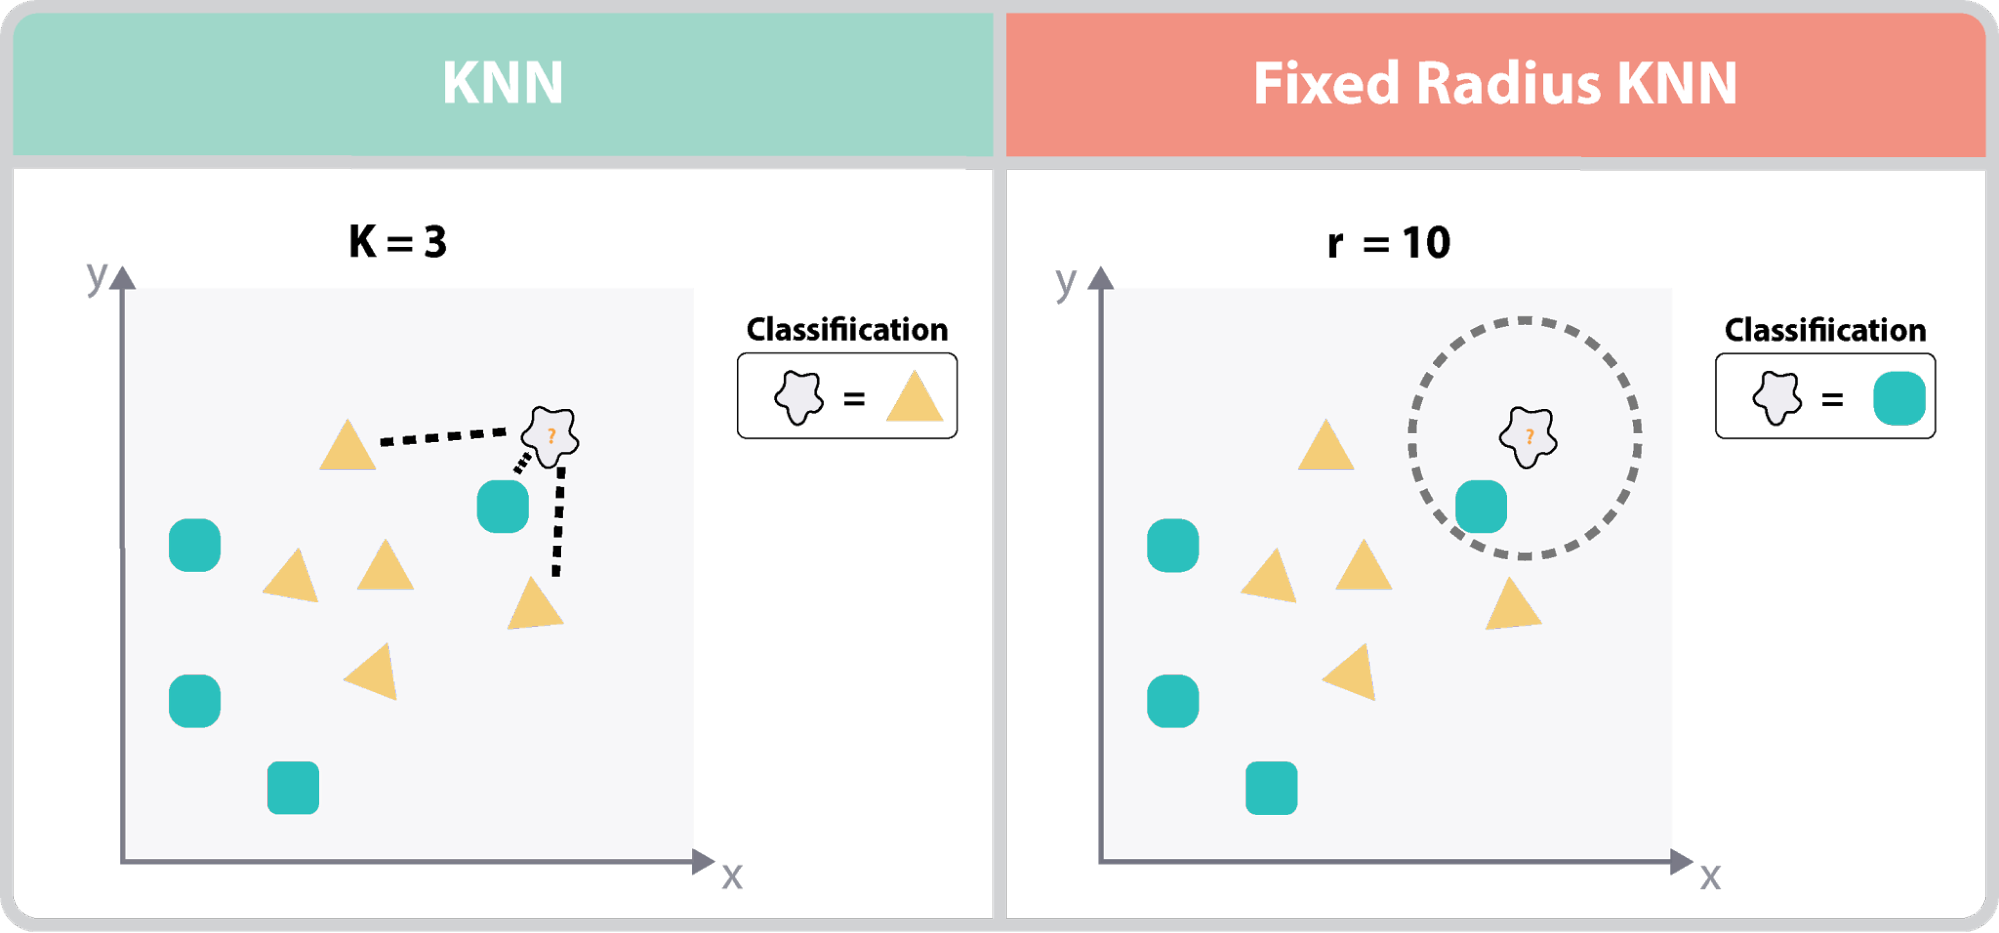
\includegraphics[width=0.5\textwidth]{image-21.png}
    \caption{k-najbliži sused i radius zasnovan najbliži sused klasifikacija za neki skup podataka}
\end{figure}

Distanca može imati bilo koju metričku meru: \textit{standardna Euklidska distanca} je najobičniji izbor. Metode zasnovane na susedima su poznate kao \textit{negeneralizujuće} metode mašinskog učenja, pošto prosto ``se sete'' svih podataka iz trening skupa (moguće transformisanih u brze sturkture indeksiranja kao što su \textit{KD Tree} ili \textit{Ball Tree} o kojima će biti reči kasnije). 

Naspram njene jednostavnosti, NN su se pokazali kao uspešni pri velikom broju klasifikacionih problema, uključujući rukopise cifara i scene satelitskih snimaka. Kao neparametarski metod, uspešno radi klasifikacije i pri neregularnim granicama odlučivanja.

Za matrice kao ulazne podatke se ustupa:
\begin{itemize}
    \item Za guste matrice, veliki broj je podržanih metrika distance.
    \item Za raspršene arbitrarne metrike Mikovskog su podržane : npr. $d_{\mathbf{p}} : (x, y) \mapsto \|x-y\|_p = \bigg(\sum_{i=1}^{n} |x_i-y_i|^p\bigg)^\frac{1}{p}$.\cite{minkowski}\cite{distance}
\end{itemize}

Tu su većina rutina obuke koje se oslanjaju na NN u njihovoj srži, kao što je \textit{procena gustina kernelom}. 

Klasifikacije zasnovane na susedu su \textit{tipa obuke zasnovane na uzorcima/instancama kao negeneralizujuće}: ne pokušava da gradi opšte unutrašnje modele, ali jednostavno skladišti uzorke trening skupa. Klasifikacija sračunava po prostom ``glasanju'' većine najbližih suseda: tačke upita dodeljene klase podataka koje imaju najviše zastupljenika od najbližih suseda tačke. 
KNN je najčešće korišćena tehnika, po kojoj od optimalnog izbora vrednosti $k$ postoji jaka zavisnost podataka - veće $k$ potiskuje efekat šuma, ali pravi ograničavanja klasifikacija manje nezastupljenim. 
Za uniformno uzorkovane podatke predlaže se NN zasnovan na radiusu, td. je lakše u situaciji kada su tačke uzoraka raspršene. Za visoku dimenzionalnost parametarskih prostora, ovaj metod postaje manje efikasan zbog \textit{``prokletstva dimenzionalnosti''}.


U nekim slučajevima je bolje \textit{udeliti težine susedima} tako da što bliži susedi doprinose više pri poklapanju obuke, a one mogu biti \textit{uniformne}, \textit{na osnovu distance} (proporcionalno inverzna distanci tačke upita) i \textit{korisnički definisana funkcija}. Priložen je primer na slici 22. koja prikazuje ponašanje težinskih faktora.

\begin{figure}[h!]
    \centering
    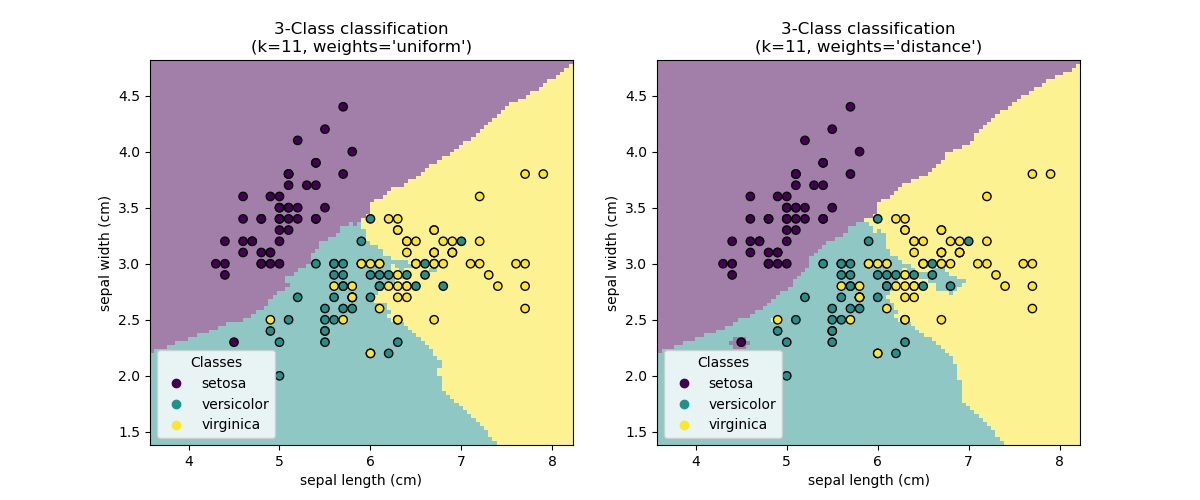
\includegraphics[width=0.75\textwidth]{image-22.png}
    \caption{\centering kNN klasifikacija skupa podataka iris od 3 klase, gde je $k=11$ u 2 slučaja težinskih faktora uniformnih i na osnovu distance}
\end{figure}

\newpage


\section{Diskusija o algoritmima}
Svaki algoriritam ima sopostvene osobine koji mogu da se iskoriste posebne probleme ili ne moraju biti baš dobar izbor za neki drugi slučaj korišćenja. Tako se uvek oslanjamo na isprobavanje drugačijih algoritama da bi se srela što bolja tačnost i pouzdan model za određen projekat, kao što je prikazano na slici 31.\cite{comparison}

\vbox{}

\subsection{Prednosti i mane algoritama, primena\cite{comp1a}\cite{comp1b}\cite{comp2}\cite{comp3}\cite{comp4}}
\subsubsection{Logistička regresija}

%https://towardsdatascience.com/comparative-study-on-classic-machine-learning-algorithms-24f9ff6ab222
% Advantages :
\textbf{Prednosti:}
\begin{itemize}
    \item Lak, brz, jednostavan klasifikacioni metod;
    \item $\beta$ parametar objašnjava smer i intenzitet važnosti nezavisnih promenljivih naspram zavisnih promenljivih;
    \item Može biti korišćen za višeklasne klasifikacije isto;
    \item Funkcija gubitka (uglavnom cross-entropija) je uvek konveksna;
    \item Vrši efikasna predviđanja na linearno separabilnim skupovima podataka;
    \item Može se izboriti sa (ne)linearnim srodnostima između features-a i cilja (možda ne?);
    \item Dobar za binarne klasifikacije;
    \item Moguća je regulacija zarad izbegavanja overfitting-a;
    \item Moguća je brza ažuriranja novim podacima.
\end{itemize}
%     Easy, fast and simple classification method.
%     θ parameters explains the direction and intensity of significance of independent variables over the dependent variable.
%     Can be used for multiclass classifications also.
%     Loss function is always convex.

% Disadvantages :
\textbf{Mane:}
\begin{itemize}
    \item Ne može biti primenjen na nelinearnim klasifikacionim problemima;
    \item Adekvatna selekcija features-a je obavezna;
    \item Očekuje se dobar SNR (signal-šum proporcija);
    \item Kolinearnost i diskiriminativnost (outliers-i) štete tačnosti modela;
    \item Moguća je samo primena diskretnih promenljivih pri predviđanju;
    \item Podleže overfitting ako je skup podataka mali;
    \item Nagađa da su features-i i ciljevi linearno srodni, što ne mora uvek da znači.
\end{itemize}

\textbf{Pogodni slučajevi primene:}
\begin{itemize}
    \item Kada odnos između features-a i cilja je jednostavan i linearan;
    \item Kada efikasnost složenosti izračunavanja je bitna.
\end{itemize}

% Logistic regression:
% -Output is a probability
\textbf{Sveukupno viđenje: (upitna tačnost)}
\begin{itemize}
    \item Izlaz je verovatnoća;
    \item Granica odluke - linearna;
    \item Osetljiva na outliers-e;
    \item Osetljiva na overfitting i underfitting (zanemarivanje objektivno značajnog broja uzoraka klase)\cite{underfitting};
    \item Nagađanja da podaci su linearni, normalizovani;
    \item Složenost modela - niska;
    \item Interpretabilnost (ne zahteva fino podešavanje od strane korisnika)\cite{interoperability} - visoka;
    \item Lakoća implementacije - visoka.
\end{itemize}
 
% -Decision boundary is linear
% -Sensitive to outliers
% -Sensitive to overfitting and underfitting
% -Data assumptions: linearity, normality
% -Model complexity: low
% -Interpretability: high
% -Ease of implementation: high
%     Cannot be applied on non-linear classification problems.
%     Proper selection of features is required.
%     Good signal to noise ratio is expected.
%     Colinearity and outliers tampers the accuracy of LR model.

% /home/zorin/Downloads/926pm_10.EPRA JOURNALS 10442.pdf
% The advantages of using Logistic Regression algorithm are:
%  It makes efficient predictions on linearly separable dataset
%  It can be used for data with multiple categories.

% The disadvantages of using Logistic Regression algorithm are:
%  It can only be used for prediction of discrete variables
%  It is prone to overfitting if the dataset is small
% https://behesht.medium.com/classification-determining-the-appropriate-model-support-vector-machine-or-logistic-regression-4a559b06244a
% Pros:
% • Simple and efficient to implement.
% • Can handle both linear and non-linear relationships between features and
% target.
% • Good for binary classification problems.

% • Can be regularized to prevent overfitting.

% • Can be updated easily with new data.

% Cons:
% • Assumes a linear relationship between features and target, which may not
% always be the case.
% • Can be sensitive to outliers.

% When to use:
% • When the relationship between features and target is simple and linear.
% • When computational efficiency is important.


% Logistic regression:
% -Output is a probability
% -Decision boundary is linear
% -Sensitive to outliers
% -Sensitive to overfitting and underfitting
% -Data assumptions: linearity, normality
% -Model complexity: low
% -Interpretability: high
% -Ease of implementation: high

\subsubsection{Stabla odlučivanja}
% https://towardsdatascience.com/comparative-study-on-classic-machine-learning-algorithms-24f9ff6ab222
\textbf{Prednosti:}
\begin{itemize}
    \item Predobrada podataka nije potrebna (pri manju parametrizacija, nedostajućim vrednostima);
    \item Nema nagađanja u vezi distribucije podataka;
    \item Obrađuje kolinearnost (uzorke duplikate)\cite{colinear} efikasno;
    \item Ustupaju dobro pojašnjenje predviđanja (mimikuju ljudsku logiku zarad toga);
    \item Efikasni u dohvatanju međusobno nelinearnih features-a podataka;
    \item Mogu raditi sa kategoričkim i numeričkim podacima;
    \item Efikasnost uspostavljena po algoritmu pretraga stabla;
\end{itemize}
% Advantages :

%     No preprocessing needed on data.
%     No assumptions on distribution of data.
%     Handles colinearity efficiently.
%     Decision trees can provide understandable explanation over the prediction.

\textbf{Mane:}
\begin{itemize}
    \item Mogućnost overfitting-a modela ako se iznova gradi stablo da bi se dosegla visoka čistost, tj. može doseći preterano veliku dubinu - za koje je uz odsecanje stabala ili korišćenje slučajnih šuma su moguća rešenja ovog problema;
    \item Štete mu outliers-i - svakim drugačijim rukovanjem njima moguće je dobiti vrlo različite oblike stabala;
    \item Može se izgraditi u veoma složen model pri radu sa komplikovanim skupovima podataka (višedimenzionalnim naspram broja features-a);
    \item Gubi vredne informacije dok radi sa kontinualnim vrednostima;
    \item Može biti previše oslonjen (da ima bias) na features-e sa vrednostima više kategorija.
    \item Znaju davati lokalno optimalne rezultate, umesto idealno globalne.
\end{itemize}

% Disadvantages :

%     Chances for overfitting the model if we keep on building the tree to achieve high purity. decision tree pruning can be used to solve this issue.
%     Prone to outliers.
%     Tree may grow to be very complex while training complicated datasets.
%     Looses valuable information while handling continuous variables.

% 2.
% he advantages of using Decision Tree Classifier are:
%  Mimic human logic and are therefore easy to interpret.
%  Efficient in capturing non-linear data patterns
%  Due to the non-parametrised approach, there is less preprocessing of the dataset.
% The disadvantages of using Decision Tree Classifier are:
%  Prone to overfitting
%  Slight variations in data can lead to completely different results
%  It becomes too complex where there are many attributes involved

% 3. 
% Pros:
% • Simple and easy to understand.
% • Can handle both categorical and numerical data.
% • Can handle non-linear relationships between features.
% • Can be used for both regression and classification problems.
% Cons:
% • Can easily overfit if the tree is too deep.

% • Can be unstable, meaning that small changes in the data can result in a
% different tree.
% • Can be biased towards features with many categories.
\textbf{Pogodni slučajevi primene:}
\begin{itemize}
    \item Kada srodnost između features-a i ciljanih vrednosti je složena i nelinearna;
    \item Interpretabilnost je važna;
\end{itemize}

\textbf{Sveukupno viđenje:}
\begin{itemize}
    \item Izlaz je labela klase;
    \item Granica odluke je nelinearna;
    \item Osetljiva na outliers-e;
    \item Osetljiva na overfitting i underfitting;
    \item Složenost modela - srednja;
    \item Nagađanja o svojstvima podatka nema;
    \item Interpretabilnost - visoka;
    \item Lakoća implementacije - visoka;
\end{itemize}
% When to use:
% • When the relationship between features and target is complex and non-linear.
% • When interpretability is important.

% Decision tree:
% -Output is a class label
% -Decision boundary is nonlinear
% -Not sensitive to outliers
% -Sensitive to overfitting and underfitting
% -Data assumptions: none
% -Model complexity: medium
% -Interpretability: high
% -Ease of implementation: high

% 4. A Comparative Analysis of Machine Learning Algorithms for
% Classification Purpose
% Vraj Sheth a , Urvashi Tripathi a , Ankit Sharma a, 2023.

% The following are some of the benefits of using a Decision Tree: It is effective for both regression and classification
% problems, with ease of interpretation, the ability to fill incomplete data in attributes with the most likely value and
% handling categorical and quantitative values. It also has a superior productivity due to the efficiency of the tree
% traversal algorithm. 

% Over-fitting is a problem that Decision Tree may experience, and the answer is Random Forest,
% which is based on an ensemble modelling technique.
% The following are the downsides of using a Decision Tree: it is being unstable, difficult to manage tree size, prone
% to errors in sampling, and providing a locally optimal answer rather than a globally ideal solution

\subsubsection{Slučajne šume}
% 1.
\textbf{Prednosti:}
\begin{itemize}
    \item Tačan i moćan model;
    \item Rukuje overfitting-om efikasno;
    \item Podržava implicitan odabir feature-a i izvodi važnost feature-a;
    \item Kombinuje više stabala, pa je pouzdaniji od stabala odlučivanja;
    \item Radi sa kategoričkim i numeričkim podacima;
    \item Efikasni u dohvatanju međusobno nelinearnih features-a podataka.
\end{itemize}

\textbf{Mane:}
\begin{itemize}
    \item Složeniji i sporiji pri izvršavanju kada šuma postane veća;
    \item Nisu dobar opisni model naspram predviđanja;
\end{itemize}
% Advantages :

%     Accurate and powerful model.
%     handles overfitting efficiently.
%     Supports implicit feature selection and derives feature importance.
% Disadvantages :

%     computationally complex and slower when forest becomes large.
%     Not a well descriptive model over the prediction.

% 2.

% 3. 
% Pros:
% • More robust than single Decision Trees, as it combines multiple trees.

% • Can handle both categorical and numerical data.
% • Can handle non-linear relationships between features.
% • Can be used for both regression and classification problems.
% Cons:
% • Can be computationally expensive.
% • Can be difficult to interpret.
\textbf{Pogodni slučajevi primene:}
\begin{itemize}
    \item Kada srodnost između features-a i ciljanih vrednosti je složena i nelinearna;
    \item Kada je overfitting problematika kod drugih klasifikatora.
\end{itemize}

\textbf{Sveukupno viđenje:}
\begin{itemize}
    \item Izlaz je labela klase;
    \item Granica odluke je nelinearna;
    \item Nije osetljiva na outliers-e (Možda da?);
    \item Nije osetljiva na overfitting i underfitting;
    \item Nagađanja o svojstvima podatka nema;
    \item Složenost modela - visok;
    \item Interpretabilnost - niska;
    \item Lakoća implementacije - visoka;
\end{itemize}
% When to use:
% • When the relationship between features and target is complex and non-linear.
% • When overfitting is a concern.

% -Output is a class label
% -Decision boundary is nonlinear
% -Not sensitive to outliers
% -Not sensitive to overfitting and underfitting
% -Data assumptions: none
% -Model complexity: high
% -Interpretability: low
% -Ease of implementation: high

\subsubsection{Naivni Bajes}

% 1. b. SVM RF NB https://medium.com/@dannymvarghese/comparative-study-on-classic-machine-learning-algorithms-part-2-5ab58b683ec0
% Advantages :



\textbf{Prednosti:}
\begin{itemize}
    \item Radi dobro sa manjim skupom podataka;
    \item Ako je korišćen model nezavisan od uslova, onda konvergira brže od drugih modela;
    \item Rukuje redudantnim features-ima (nepoznatim vrednostima);
    \item Podržava binarne i multiklasifikatorne probleme klasfikacija;
    \item Lak pri implementaciji;
    \item Može rukovati podacima visokedimenzionalnosti;
    \item Dobar za probleme klasifikacije teksta;
    \item Radi sa ili kategoričkim ili numeričkim podacima;
    \item Pravi dobre stohastičke preporuke.
\end{itemize}

\textbf{Mane:}
\begin{itemize}
    \item Očekuje da features-i budu strogo međusobno nezavisni - što nije baš primenljivo u stavrnom životu;
    \item Uzorci trening skupa velike brojnosti i $P(X = feature|Y) = 0$ za feature, posterior može postati $0$. Što nahodi da taj uzorak može biti loš zastupnik u populaciji - tj. osetljiv na redudantne vrednosti;
    \item Kontinualne promenljive su sumirane segmentima (binning) da ukažu na diskretne vrednosti features-a. Ovaj zadatak je neophodno raditi pažljivo da ne bi došlo do gubitka podataka i netačnosti.
    \item Previše su jednostavni modeli;
    \item Nije pogodan u višedimenzionalnim slučajevima;
    \item Vreme izvršavanja je složenije pri predviđanju naspram SVM i logističke regresije.
\end{itemize}
%     works well with less training data.
%     If NB conditional independence is satisfied, it converges faster than other discriminative models.
%     Handles irrelevant features.
%     Supports binary and multi-class classification problems.

% Disadvantages :

%     expects the features to be strictly independent to each other, which is not applicable in real life scenarios.
%     While training sample of a large population, and if we have a feature with P(X=feature|Y) as zero, the posterior probability will become zero. This happens when the sample is not representing the population properly.
%     continuous variables are binned to extract discrete values from features. This task should be carefully done to avoid data loss.
% When to Use :

%     Naive bayes is preferred when the features are mutually independent and have limited training data.
%     Naive bayes is highly used in text classification, spam filtering, recommender systems etc.

% 2. 

% 3. 
% Pros:
% • Simple and efficient to implement.
% • Can handle large amounts of data with high dimensionality.
% • Good for text classification problems.
% Cons:
% • Assumes independence between features, which may not always be the case.
% • Can be sensitive to irrelevant features.
\textbf{Pogodni slučajevi primene:}
\begin{itemize}
    \item Kada su features-i međusobno nezavisni i imaju ograničenja trening skupa podataka;
    \item Pri klasifikaciji teksta, spam filtriranja, sistema preporuka, itd.
    \item Kada su visokodimenzionalni? - Ne baš.
\end{itemize}

\textbf{Sveukupno viđenje:}
\begin{itemize}
    \item Izlaz je labela klase;
    \item Granica odluke je linearna;
    \item Nije osetljiva na outliers-e;
    \item Nije osetljiva na overfitting i underfitting;
    \item Nagađanja o svojstvima podatka je u vezi nezavisnosti;
    \item Složenost modela - niska;
    \item Interpretabilnost - visoka;
    \item Lakoća implementacije - visoka;
\end{itemize}
%!!!!!!!When to use:
% • When the data is high-dimensional and consists of text.

% Naive bayes:
% -Output is a class label
% -Decision boundary is linear
% -Not sensitive to outliers
% -Not sensitive to overfitting and underfitting
% -Data assumptions: independence
% -Model complexity: low
% -Interpretability: high
% -Ease of implementation: high

% 4.
% Naive Bayes is easy to set up, produces good results, scales proportionally with the number of predictors and data

% points, requires less training data, manages discrete and continuous data, can tackle binary and multi-class
% classification problems, and makes stochastic recommendations. Data can be processed in a continuous or
% discontinuous manner. It is unaffected by non-essential features. Naive Bayes assumes conditional independence,
% means the relationship between all input features are independent.


% The following are the drawbacks of naive Bayes: Naive Bayes models are too simplistic, models that have been
% properly trained and optimised often outperform them. If one of the features is required to be a "continuous variable"
% (such as time), it is complicated to implement Naive Bayes effectively. Even if "buckets" for "continuous variables"
% can be created, they are not 100% accurate. Because there is no genuine online option for Naive Bayes, all data must
% be saved in order to retrain the model. When the number of attributes is really high, such as > 100K, it will not scale.
% In comparison to SVM or simple logistic regression, it requires higher runtime memory for prediction. It consumes
% much time to compute, especially for models with a lot of variables.

\subsubsection{Metode potpornih vektora (SVM)}
% 1. b.

\textbf{Prednosti:}
\begin{itemize}
    \item Koristi kernel trik da ustupi kompleksna rešenja;
    \item Koristi funkciju konveksne oprimizacije kojom se uvek dostiže globalni minimum;
    \item Hindž gubici su visoke tačkosti;
    \item Outliers-i mogu biti obrađeni korišćenjem mekših margina konstantom $C$;
    \item Rade sa visokodimenzionalnim podacima;
    \item Efikasni u dohvatanju međusobno nelinearnih features-a podataka.
    \item Rade dobro sa malim skupovima podataka.
\end{itemize}

\textbf{Mane:}
\begin{itemize}
    \item Hindž gubitak vodi u raspršenost;
    \item Hiperparametrima i kernelima je važno pažljivo raditi podešavanja za podnošljivu tačnost;
    \item Većim skupovima podataka duže je vreme obuke;
    \item Interpretabilnost složenija;
    \item Može biti osetljiva na odabir parametara regularizacije $C$ (što je teško za utvrditi), i kernela;
    \item Sračunavanja verovatnoća nisu ustupljene ovim modelom.
\end{itemize}
% Advantages:

%     SVM uses kernel trick to solve complex solutions.
%     SVM uses a convex optimization function, due to which global minima is always achievable.
%     Hinge loss provides higher accuracy.
%     Outliers can be well handled using soft margin constant C.

% Disadvantages:

%     Hinge loss leads to sparsity.

%     Hyper parameters and kernels are to be carefully tuned for sufficient accuracy.
%     Longer training time for larger datasets.

% 2.

% 3. 
% Pros:
% • Can handle high-dimensional data.
% • Can handle non-linear relationships between features.
% • Can be used for both regression and classification problems.
% • Good for small datasets.
% Cons:
% • Can be computationally expensive for large datasets.

% • Can be difficult to interpret.
% • Can be sensitive to the choice of kernel and regularization parameter.
\textbf{Pogodni slučajevi primene:}
\begin{itemize}
    \item Kada srodnost između features-a i ciljanih vrednosti je složena i nelinearna;
    \item Kada se radi sa manjim skupom podataka.
\end{itemize}

\textbf{Sveukupno viđenje:}
\begin{itemize}
    \item Izlaz je labela klase;
    \item Granica odluke je nelinearna;
    \item Nije osetljiva na outliers-e;
    \item Osetljiva na overfitting i underfitting;
    \item Nagađanja o svojstvima podatka nema;
    \item Složenost modela - visoka;
    \item Interpretabilnost - niska;
    \item Lakoća implementacije - niska;
\end{itemize}
% When to use:
% • When the relationship between features and target is complex and non-linear.
% • When the dataset is small.

% SVM:
% -Output is a class label
% -Decision boundary is nonlinear
% -Not sensitive to outliers
% -Sensitive to overfitting and underfitting
% -Data assumptions: none
% -Model complexity: high
% -Interpretability: low
% -Ease of implementation: low

% 4.
% SVM has a number of limitations, including the following: Because of the longer training time, it performs poorly
% when working with large data sets. The correct kernel function will be tough to locate. When a dataset is noisy, SVM
% does not perform well. Probability calculations are not provided by SVM. It's difficult to interpret the final SVM
% model
\subsubsection{k-Najbližih suseda}
% 1. a.

\textbf{Prednosti:}
\begin{itemize}
    \item Lak za izgradnju i jednostavan za razumevanje model mašinskog učenja;
    \item Malo hiperparametara za podešavanje;
    \item Laka implementacija;
    \item Dobar za male skupove podataka;
    \item Koristan pri klasifikaciji višelabelnim vrednostima klasa;
    \item 2 puta bolje ustanovljavanje netačnosti naspram naivnih Bajesa;
    \item Npr. pri utvrđivanju svojstava proteina, profili istaknuti su bolje na osnovu funkcija, time prednjači naspram SVM pristupa.
\end{itemize}

\textbf{Mane:}
\begin{itemize}
    \item $k$ je neophodno pažljivo odabrati;
    \item Viša složenost izračunavanja ako je ogroman broj uzoraka;
    \item Neophodno je skaliranje predobradom features-a, da bi ulaz bio podnošljiv;
    \item Ostetljiv na redudantne features-e, klasifikacija nepoznatih vrednosti je skuplja;
    \item Zahteva sračunavanja distanci $k$ suseda;
    \item Tačnost ispašta šumom i redudantnim vrednostima ;
\end{itemize}
% Advantages :

%     Easy and simple machine learning model.
%     Few hyperparameters to tune.

% Disadvantages :

%     k should be wisely selected.
%     Large computation cost during runtime if sample size is large.
%     Proper scaling should be provided for fair treatment among features.

% 2. 
% The advantages of using K-Nearest Neighbors algorithm are:
%  Easy to implement
%  The model can be used for both- classification and regression problems
%  No complexity in making the model
% The disadvantages of using K-Nearest Neighbors algorithm are:
%  The model becomes slow with increasing data
%  Other models are faster and predict better results with large sets of data

% 3.
% Pros:
% • Simple and intuitive to understand.
% • Good for small datasets.
% • Can handle both categorical and numerical data.
% Cons:
% • Can be computationally expensive for large datasets.
% • Can be sensitive to irrelevant features.
\textbf{Pogodni slučajevi primene:}
\begin{itemize}
    \item Kada je skup podataka manji;
    \item Kada je interoperabilnost važna.
\end{itemize}

\textbf{Sveukupno viđenje:}
\begin{itemize}
    \item Izlaz je labela klase;
    \item Granica odluke je nelinearna;
    \item Osetljiva na outliers-e;
    \item Nije osetljiva na overfitting i underfitting;
    \item Nagađanja o svojstvima podatka nema;
    \item Složenost modela - niska;
    \item Interpretabilnost - visoka;
    \item Lakoća implementacije - visoka;
\end{itemize}
% When to use:
% • When the dataset is small.
% • When interpretability is important

% K-nearest:
% -Output is a class label
% -Decision boundary is nonlinear
% -Sensitive to outliers
% -Not sensitive to overfitting and underfitting
% -Data assumptions: none
% -Model complexity: low
% -Interpretability: high
% -Ease of implementation: high

% 4.

% Advantages of KNN algorithm are the following: It is a simple technique that may be implemented quickly. It is
% inexpensive to construct the model. It's a very adaptable categorisation technique that's ideal for Multi-modal classes.
% There are several class labels on the records. The mistake rate is twice as high as the Bayes error rate. It is sometimes
% the most effective way. When it came to predicting protein, function based on expression profiles, KNN outperformed
% SVM.

% Disadvantages of KNN are the following: It is relatively costly to classify unknown records. It requires calculating
% the distance between k-nearest neighbours. The algorithm becomes more computationally costly as the size of the
% training set grows. Accuracy will degrade as a result of noisy or irrelevant features

\begin{figure}[h!]
    \centering
    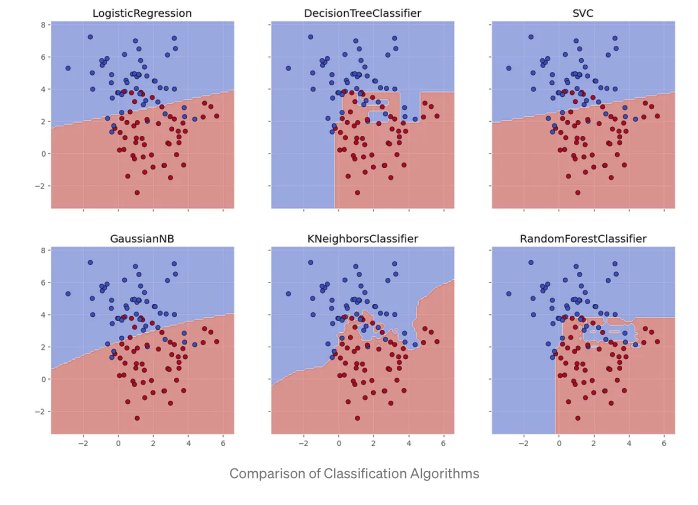
\includegraphics[width=0.9\textwidth]{image-34.png}
    \caption{Poređenje klasifikacija određenih modela}
\end{figure}
%%%%%%%%%%%%%%%%%%%%%%%%%%%%%%%%%%%%%%%%%%%%%%%%%%%%%%%%%%%%%%S
\subsection{Poređenje među algoritmima\cite{comp1a}\cite{1b}}

Radiće se kombinacije po redosledu : LR, Stabla odlučivanja, kNN, SVM, a pritom NB će već biti obrađen.

\subsubsection{Logistička regresija}
\textbf{Logistička regresija vs SVM}:
\begin{itemize}
    \item Sveukupno viđenje:SVM rukuje nelinearnim rešenjima, dok logistička regresija linearnim;
    \item Sveukupno viđenje:Linearni SVM rukuje bolje outliers-ima, kako izvodi rešenje maksimalne margine;
    \item Sveukupno viđenje:Hidž sračunat gubitak kod SVM-a prevazilazi log loss kod logističke regresije.
\end{itemize}

\textbf{Logistička regresija vs Stablo odlučivanja}
\begin{itemize}
    \item Sveukupno viđenje:Stabla odlučivanja rukuju kolinearnošću bolje nego logistička regresija.
    \item (bolji) Stabla odlučivanja ne mogu izvesti važnosti features-a, ali logistička regresija može;
    \item Sveukupno viđenje:Stabla odlučivanja se pokazuju bolje pri radu nad kategoričkim vrednostima od logističke regresije.
\end{itemize}

\textbf{Logistička regresija vs Naivni Bajes}
\begin{itemize}
    \item NB je generativni model gde LR je diskiriminativni;
    \item NB radi dobro sam malim skupovima podataka, gde LR uz regularizaciju možde dostići slične performanse;
    \item LR radi bolje od NB pri slučaju kolinearnosti, dok NB očekuje da svi features-i budu nezavisni.
\end{itemize}

\textbf{Logistička regresija vs kNN}
\begin{itemize}
    \item kNN je neparametarski model, dok LR je parametarski model;
    \item kNN je uporedivo sporiji od LR;
    \item kNN podržava nelinarna rešenja dok LR podržava samo linearna;
    \item LR može generisati nivo pouzdanosti predviđanja, dok kNN samo 
\end{itemize}

\subsection{Stabla odlučivanja}
Sličan ishod upoređivanja Stabla odlučivanja je i za upoređivanje sa Slučajnim šumama, ali evo poređenja ova dva.

\textbf{Stabla odlučivanja vs Slučajne šume}
\begin{itemize}
    \item Slučajna šuma je skupina stabala odlučivanja i prosečno/većinsko glasanje šume je uzeto kao ishodujuće predviđanje;
    \item Slučajna šuma je manje oštećen overfitting-om od stabla odlučivanja, da je više generalizovanije rešenje;
    \item Slučajna šuma je pouzdanija i tačnija od stabla odlučivanja.
\end{itemize}

\textbf{Stabla odlučivanja vs Naivni Bajes}
\begin{itemize}
    \item Stablo odlučivanja je diskiriminativni model, gde Naivni Bajes je generativni;
    \item Stablo odlučivanja je fleksibilniji i lakši;
    \item Stablo odlučivanja uz odsecanje mogu zanemariti ključne vrednosti pri obuci podataka, što tačnost dovodi u rizik.
\end{itemize}

\textbf{Stabla odlučivanja vs SVM}
\begin{itemize}
    \item SVM koristi kernel trik da reši probleme nelinearnosti dok stablo odlučivanja koristi hiper-pravougaonike da bi rešio problem ulaznog prostora;
    \item Stbla odlučivanja su bolja za kategoričke podatke i rukuju sa kolinearnostima bolje od SVM-a.
\end{itemize}

\textbf{Stablo odlučivanja vs kNN}
\begin{itemize}
    \item Oba su neparametarski metodi;
    \item Stablo odlučivanja ima podršku za automatsku interakciju feature-a, dok kNN nema.
    \item Stablo odlučivanja je brže od kNN-ovog skupog vremenski složenog izvršavanja.
\end{itemize}

\subsubsection{$k$-Najbližih suseda(kNN)}
\textbf{kNN vs NB}
\begin{itemize}
    \item NB je mnogo brži od kNN po vremenskoj složenosti;
    \item NB je parametarski, dok kNN je neparametarski.
\end{itemize}

\textbf{kNN vs SVM}
\begin{itemize}
    \item SVM brine više  o outliers-ima nego kNN;
    \item Ako trening skup $n_{uzoraka} >> n_{features}$, kNN je bolji od SVM, inače SVM prevazilazi kNN.
\end{itemize}

\subsubsection{Metode potpornih vektora (SVM)}
\textbf{SVM vs Slučajna šuma}
\begin{itemize}
    \item Slučajna šuma podržava višeklasne klasifikacije, gde SVM mora da obezbedi više modela za to;
    \item Slučajna šuma daje verovatnoću naspram predviđanja, dok SVM to ne radi;
    \item Slučajna šuma rukuje bolje kategoričkim podacima od SVM.
\end{itemize}

\textbf{SVM vs NB}
\begin{itemize}
    \item Oba rade bolje sa manjim trening skupom i većim brojem features-a;
    \item Ako su međusobno zavisni features-i, SVM prevazilazi NB;
    \item SVM je diskiriminativni model, dok NB je generativni model.
\end{itemize}

\subsubsection*{Dodatna sagledanja\cite{comparison}}
Za \textbf{brzinu pri obuci} oslanja se na LR, NB klasifikatore (slučajne šume su spore za to). kNN je uporedivo \textbf{generalno sporiji} od LR, NB i sporiji od stabala odlučivanja. 

kNN je skup što se tiče \textbf{memorije pri obuci} pošto mora da vodi računa o svim trening podacima i o tome da treba da nađe čvorove suseda.

NB radi dobro sa malim skupovima podataka.

\textbf{Fleksibilnost} nije prisutna kod LR toliko da može da uhvati složenije srodnosti features-a. Stablo odlučivanja podržava nelinearnost. SVM podržava oba (ne)linearna rešenja.
kNN je bolji od LR kada podaci imaju visok SNR.
Slučajne šume su pouzdanije i tačnije od stabala odlučivanja.

\newpage

\section{Zaključak}

Na početku su pokušana izlaganja objašnjenja za stukturu skupa podataka uz razjašćanjavanje (šta je učenje, šta se najčešće koristi, šta su zahtevi rada pri nadgledanom učenju) i postepeno razgraničenje pojmova sadržanih (uzorak, atribut/feature, labela po brojnosti, klasa po brojnosti, trening i test skup), načina obuke sve do klasifikacija.

\vbox{}

U teorijskim osnovama i metodologijama redom su istaknute teme logičke regresije, stabla odlučivanja, slučajne šume, naivnog Bajesa, SVM i kNN-a. 

\vbox{}


Za logičku regresiju pomenuti su koncepti logit funkcije (logaritam neobičnosti) uz linearne kombinacije kojom može se predstaviti, klasifikacije maksimuma entropije zasnovanom na verovatnoći i na slučajnom odabiru uzorka, log-linearnom klasifikatorom koji je nalik logit funkciji samo preoblikovanom, pa onda podela na verovatnoće ishoda tipa binarna (koeficijenta regulacije, korisnički dodeljenih težina uzoraka/klase, funkcija procene) i OVR, a tu su multiunomijalne logističke regresije (po log-linearnim modelima, prekomerne parametrizacije i simetričnog induktivnog bias-a, optimizacije), kao $l_1, l_2$ i regularizacija elastične mreže. 

\vbox{}


Za stabla odlučivanja koji je uvelo pojmove neparametarskog obučavanja, isparčane konstantne aproksimacije, pravila odlučivanja (dato if-then-else), pomenuto smanjenje dimenzionalnosti uz PCA (uz njega rastuće ortogonalne komponente, ICA, feature selection procesi), dat je uvid u slučaju multilabel problema i predstavljen je koncept istovremenog predviđanja, dat je primer njegove upotrebe pri upotpunjavanju dela slike lica na osnovu predviđanja. Data je analiza složenosti i pojma balansiranog stabla, podstabla (aproksimativno) balansirajućeg, kriterijum nečistosti, logaritamski gubitak, information gain.  Data matematička formulacija kao predstavljanje metodologije, uz principe podele praga, funkcije gubitka(gini, entropija/log-loss), kriterijuma klasifikacije, Shannon entropije, cross-entropije. Predstavljen je koncept obrade nepostojanih vrednosti (pri nailazećim podelama, neizvesnosti, itd.). Rešenje dato za problem situacije overfitting-a kao što je odsecanje minimalnom cenom složenosti i parametra za postavljanje $ccp_alpha$.

\vbox{}


Za slučajne šume kao metod ansambla ukazano je na to da se oslanjaju na ustanovljavanje proseka tačnosti i upravljanja overfitting-a. Uključeni su koncepti ``pomešati i kombinovati'', koncept nasumičnosti, bootstrap uzorka. Ukazuje se blag na porast   cene u bias-u.  Ukazivanje na parametre brojnosti komponenti stabla i ishoda, ukazivanje na rešenje cross-validation-om. Daje se uvid u bootstrap bagging agregacije za procenjivanje grešaka generalizacija. Ističe se pojam važnosti feature-a (pominje se za feature selection mera središnjeg opadanja u nečistosti MDI i ukazuje se na 2 zablude i među njima se ukazuje na koncept permutacije važnosti features-a). 

\vbox{}


Za klasifikaciju naivnim Bajesom ukazuje se na pojmove Bajesove teoreme i naivnim pretpostavkama. Bitni koncepti su prior, evidence, likelihood, posterior verovatnoće, nezavisnosti događaja, uslovne nezavisnosti, verovatnoća maksimalnog a posteriori - MAP, Gausova verzija - koja koristi koncepte Gausove distribucije, i verovatnoće maksimalne verodostojnosti - MLE, multinomijalna (MNB) verzija za 2 ili više vrednosti nezavisnih features-a uz parametar smooth-ovanja MLE-a (slučaja Laplace i Lidstone), komplementarni naivni bajes (CNB) kao proširenjem MNB-a, Bernulijeva verzija (BNB) koji koristi višestruku Bernilijevu distribuciju koji eksplicitno kažnjava neispoljavanje feature-a, i kategorički NB je zasnovan na kategoričkoj distribuciji. Dat je uvid u problem klasifikacije velikih razmera i koncepta out-of-core klasifikacije.

\vbox{}


Za metode potpornih vektora (SVM) dat je uvid u njegove karakteristike, verzije nu-SVM, linearnog SVM-a kom je udeljen linearni kernel, gubici kvadratnih hindževa, kombinacija  LIBLINEAR rešavačima, skaliranja presecanja, finetunning slujave, verziju SVM-a koji je nelinearan RBF kernelom i koji rešava problem linearne nesaparabilnosti. Dalje se pominju težinskih faktora klase i uzoraka, kvadratnog programerskog problema kao srži SVM-a, itd. Date su kernel funkcije linearnba, polinomijalne, Radial-basis funkcija - RBF (koja sa sobom zahteva 2 parametra: $C$ za regularizaciju, tj. izbegavanje uzoraka koji loše se klasifikujum; $\gamma$ za ustanovljavanja uticaja jednog uzorka), sigmoidna, mogućnost prepravljanja funkcija kernela uz korišćenje Gram matica. Potom se ide na glavnu stvar gde se pominju bitni koncepti hiperravni, funkcionalna margina separacija uzoraka, granica margine, potpornih vektora, glavnog problema maksimizovanja margina, kažnjavanja, parametra izverzne regularizacije, sporednog problema, kernela, dualnih koeficijenata, kernel trika $\phi$, funkcije odlučivanja kao problema optimizacije, itd. Za linearni SVM klasifikator se pominje njegov glavni problem za rešavanje, primena hindž funkcije gubitka, nekorišćenje kernel trika. Priče o verziji nu-SVM-a uspostavljanja gornje granice frakcija gešaka i donje granice frakcija potpornih vektora.

\vbox{}

Za kNN je ustanovljen princip nalaženja broja najbližih suseda trening uzoraka u odstojanju od tačke novog uzorka, gde je $k$ unapred korisnički postavljena brojka ili samo zavisi od radijusa (poluprečnika) korisnički postavljenog $r$. Obraća se pažnja na indeksiranja pri transoformisanja negeralizujuće metode, primenu kod rukopisa cifara, scene satelitskih snimaka. Naglašava se da je neparametarski i radi klasifikacije u neregularnim granicama odlučivanja gusta, raspršena; da se vrše procena gustina kernelom kao srž većina NN rutina. slučaja negeralizujuće obuke i skladištenja, tačke upita, koncepta glasanja, prokletstva dimenzionalnosti, težina udeljenih susedima. 

\vbox{}

U 3. sekciji obavljena je diskusija algoritama šta su povoljnosti, šta nepogodnosti (težina implementacije, brzina izvršavanja, jednostavnost interpretacije, inteoperabilnost, povoljnost parametara koji se podešavaju unapred, adekvatnost funkcija gubitaka, kakav je odnos na linearnu separabilnost, itd.), situacija kada je poželjna primena, sveukupno sagledanje (vrsta vrednosti izlaza labele, linearnost granica odluke, osetljivost na outliers-e, osetljivost na underfitting i overfitting, složenost modela, nagađanja o svojstvima podataka, interoperabilnost, lakoću implementacije) za svaki opšte pomenut algoritam.

Dalje su data neka usoprotstavljena poređenja algoritama po nekim osobinama (gori, nerešeno, bolji).

%%%%%%%%%%%%%%%%%%%%%%%%%%%%%%%%%%%%%%%%%%%%%%%%%%%%%%%%%%%%%%
% \begin{figure}[h!]
%     \centering
%     \includegraphics[width=0.5\textwidth]{neuron}
%     \caption{Veštački neuron}
% \end{figure}

%%%%%%%%%%%%%%%%%%%%%%%%%%%%%%%%%%%%%%%%%%%%%%%%%%%%

% \cite{humancpu}

% \subsection{\normalsize{Pogled na pojmove inteligencije, znanja, ljudske imitacije}}
% \subsubsection{\normalsize{Istorija temelja veštačke inteligencije}}



% \begin{enumerate}
    % \item [3.]{\textbf{Da li uticaj misli tradicionalnog zapadnog sveta obazirale su se nad pitanjem odnosa tela i uma kao: 
    % bla bla

    % \item[5.] {\textbf{Moja lična zahtevanja oko inteligencije računarkog softvera.}}
    % bla bla

% \end{enumerate}
\newpage

\begin{thebibliography}{1}
    % \bibitem{texbook}
    % Donald E. Knuth (1986) \emph{The \TeX{} Book}, Addison-Wesley Professional.
    % \bibitem{lamport94}
    % Leslie Lamport (1994) \emph{\LaTeX: a document preparation system}, Addison
    % Wesley, Massachusetts, 2nd ed.
    \bibitem{supervised}
  An introduction to machine learning with scikit-learn, \url{https://scikit-learn.org/stable/tutorial/basic/tutorial.html}, Datum poslednjeg pristupa: \today
  \bibitem{semi}
  Semi-supervised learning, \url{https://scikit-learn.org/stable/modules/semi_supervised.html}, Datum poslednjeg pristupa: \today
  \bibitem{rl}
  Introduction to RL and Deep Q Networks, \url{https://www.tensorflow.org/agents/tutorials/0_intro_rl}, Datum poslednjeg pristupa: \today
  \bibitem{algs}
  5 Classification Algorithms for Machine Learning, \url{https://builtin.com/data-science/supervised-machine-learning-classification}, Datum poslednjeg pristupa: \today
    \bibitem{logit}
    R Documentation, The logit and inverse-logit functions, \url{https://search.r-project.org/CRAN/refmans/LaplacesDemon/html/logit.html}, Datum poslednjeg pristupa: \today
    \bibitem{logit2}
    Understanding Logit: The Link Function in Logistic Regression, \url{https://deepai.org/machine-learning-glossary-and-terms/logit}, Datum poslednjeg pristupa: \today
    \bibitem{entropy}
    JavaTpoint, Entropy in Machine Learning \url{https://www.javatpoint.com/entropy-in-machine-learning}, Datum poslednjeg pristupa: \today
    \bibitem{loglinear}
    Soczewica R., 2021., When should we use the log-linear model?, \url{https://towardsdatascience.com/when-should-we-use-the-log-linear-model-db76c405b97e}, Datum poslednjeg pristupa: \today
    \bibitem{onerest}
    Brownlee J., 2021., One-vs-Rest and One-vs-One for Multi-Class Classification, \url{https://machinelearningmastery.com/one-vs-rest-and-one-vs-one-for-multi-class-classification/}, Datum poslednjeg pristupa: \today
    \bibitem{symmetry}
    Raman N., Magazzeni D., Shah S. 2023., Bayesian Hierarchical Models for Counterfactual Estimation, Figure 4, \url{https://www.researchgate.net/figure/Inductive-bias-in-categorical-values-of-generated-counterfactuals-left-Posterior_fig2_367359800}, Datum poslednjeg pristupa: \today
    \bibitem{overparametrization}
    Schmidt M.,  Le Roux N.,  Bach F., Minimizing Finite Sums with the Stochastic Average
Gradient. Mathematical Programming, 2017, 162 (1-2), pp.83-112. 10.1007/s10107-016-1030-6. hal-
00860051v2, \url{https://inria.hal.science/hal-00860051/document}, Datum poslednjeg pristupa: \today
    \bibitem{lrsolvers}
    sklearn linear model LogisticRegression, \url{https://scikit-learn.org/stable/modules/generated/sklearn.linear_model.LogisticRegression.html#sklearn.linear_model.LogisticRegression}, Datum poslednjeg pristupa: \today
    \bibitem{liblinear}
    Rong-En Fan, Kai-Wei Chang, Cho-Jui Hsieh, Xiang-Rui Wang, Chih-Jen Lin, 2022., LIBLINEAR: A Library for Large Linear classification
    \bibitem{sag}
    P.J.T. Notsawo, 2023., Stochastic Average Gradient : A Simple Empirical Investigation, description \url{https://arxiv.org/abs/2310.12771}, Datum poslednjeg pristupa: \today
    \bibitem{sag}
    Defazio A., Bach F. 2014., SAGA: A Fast Incremental Gradient Method With Support for Non-Strongly Convex Composite Objectives, description \url{https://arxiv.org/abs/1407.0202v3}, Datum poslednjeg pristupa: \today
    \bibitem{bfgs}
    Gilles-Philippe Paillé,2019., SciPy optimisation: Newton-CG vs BFGS vs L-BFGS, \url{https://stackoverflow.com/questions/42424444/scipy-optimisation-newton-cg-vs-bfgs-vs-l-bfgs}, Datum poslednjeg pristupa: \today
    \bibitem{nc}
    J. Bräuninger, 1980., A quasi-Newton method with Cholesky factorization, description \url{https://link.springer.com/article/10.1007/BF02259641}, Datum poslednjeg pristupa: \today
    \bibitem{dtrees}
    1.10. Decision Trees, \url{https://scikit-learn.org/stable/modules/tree.html#tree-algorithms-id3-c4-5-c5-0-and-cart}, Datum poslednjeg pristupa: \today
    \bibitem{wbox}
    Difference between Black Box Vs White Vs Grey Box Testing, \url{https://www.geeksforgeeks.org/difference-between-black-box-vs-white-vs-grey-box-testing/}, Datum poslednjeg pristupa: \today
    \bibitem{extrapolation}
     Awati R., 2022., extrapolation and interpolation, \url{https://www.techtarget.com/whatis/definition/extrapolation-and-interpolation}, Datum poslednjeg pristupa: \today
     \bibitem{np}
     baeldung, 2022., P, NP, NP-Complete and NP-Hard Problems in Computer Science, \url{https://www.baeldung.com/cs/p-np-np-complete-np-hard}, Datum poslednjeg pristupa: \today
     \bibitem{xor}
     Is there a proof to explain why XOR cannot be linearly separable?, \url{https://ai.stackexchange.com/questions/25228/is-there-a-proof-to-explain-why-xor-cannot-be-linearly-separable}, Datum poslednjeg pristupa: \today
     \bibitem{sieve}
     Open question: The parity problem in sieve theory, \url{https://terrytao.wordpress.com/2007/06/05/open-question-the-parity-problem-in-sieve-theory/}, Datum poslednjeg pristupa: \today
     \bibitem{pca}
     2.5.1. Principal component analysis (PCA), \url{https://scikit-learn.org/stable/modules/decomposition.html#pca}, Datum poslednjeg pristupa: \today
     \bibitem{ica}
     2.5.6. Independent component analysis (ICA), \url{https://scikit-learn.org/stable/modules/decomposition.html#independent-component-analysis-ica}, Datum poslednjeg pristupa: \today
     \bibitem{fs}
     1.13. Feature selection, \url{https://scikit-learn.org/stable/modules/feature_selection.html#feature-selection}, Datum poslednjeg pristupa: \today
     \bibitem{ccpalpha}
     Post pruning decision trees with cost complexity pruning, \url{https://scikit-learn.org/stable/auto_examples/tree/plot_cost_complexity_pruning.html#sphx-glr-auto-examples-tree-plot-cost-complexity-pruning-py}, Datum poslednjeg pristupa: \today
     \bibitem{rf}
     sklearn.ensemble.RandomForestClassifier, \url{https://scikit-learn.org/stable/modules/generated/sklearn.ensemble.RandomForestClassifier.html}, Datum poslednjeg pristupa: \today
     \bibitem{pnc}
     Tixier A.J.P., 2018., Perturb and Combine to Identify Influential
Spreaders in Real-World Networks, \url{https://arxiv.org/pdf/1807.09586.pdf}, Datum poslednjeg pristupa: \today
    \bibitem{cv}
    Brownlee J., 2023. A Gentle Introduction to k-fold Cross-Validation, \url{https://machinelearningmastery.com/k-fold-cross-validation/}, Datum poslednjeg pristupa: \today
    \bibitem{ensamblerf}
    1.11.2. Random forests and other randomized tree ensembles, \url{https://scikit-learn.org/stable/modules/ensemble.html#forest}, Datum poslednjeg pristupa: \today
    \bibitem{permutation}
    4.2. Permutation feature importance, \url{https://scikit-learn.org/stable/modules/permutation_importance.html#permutation-importance}, Datum poslednjeg pristupa: \today
    \bibitem{1ok}
    6.2. Feature extraction, \url{https://scikit-learn.org/stable/modules/feature_extraction.html}, Datum poslednjeg pristupa: \today
    \bibitem{nb}
    1.9. Naive Bayes, \url{https://scikit-learn.org/stable/modules/naive_bayes.html}, Datum poslednjeg pristupa: \today
    \bibitem{nb-names}
    Naïve Bayes Classifier, UC Business Analytics R Programming Guide, \url{https://uc-r.github.io/naive_bayes}, Datum poslednjeg pristupa: \today
    1.4.4 Conditional Independence, \url{https://www.probabilitycourse.com/chapter1/1_4_4_conditional_independence.php}, Datum poslednjeg pristupa: \today
    \bibitem{gaus}
    Pathak M., Normal Distribution, \url{https://www.kaggle.com/code/themrityunjaypathak/normal-distribution?scriptVersionId=156424946}, Datum poslednjeg pristupa: \today
    \bibitem{multinomial}
    Hosch L.W., 2024., multinomial distribution, Brittanica, \url{https://www.britannica.com/science/multinomial-distribution}, Datum poslednjeg pristupa: \today
    \bibitem{bernoulli}
    Notes: Bernoulli, Binomial, and Geometric Distributions, \url{https://my.eng.utah.edu/~cs3130/lectures/L07-BernoulliBinomialGeometric.pdf}, Datum poslednjeg pristupa: \today
    \bibitem{ordinal}
    sklearn.preprocessing.OrdinalEncoder, \url{https://scikit-learn.org/stable/modules/generated/sklearn.preprocessing.OrdinalEncoder.html#sklearn.preprocessing.OrdinalEncoder}, Datum poslednjeg pristupa: \today
    \bibitem{svm}
    1.4. Support Vector Machines, \url{https://scikit-learn.org/stable/modules/svm.html#}, Datum poslednjeg pristupa: \today
    \bibitem{knn}
    1.6. Nearest Neighbors, \url{https://scikit-learn.org/stable/modules/neighbors.html}, Datum poslednjeg pristupa: \today
    \bibitem{hinge}
    Kumawat N., 2020., Hinge Loss and Square Hinge loss,  InsideAIML, \url{https://insideaiml.com/blog/Hinge-Loss-and-Square-Hinge-loss-1068}, Datum poslednjeg pristupa: \today
    \bibitem{intercept-scaling}
    \textmd{sklearn linear model LogisticRegression - intercept scaling argument}, \url{https://scikit-learn.org/stable/modules/generated/sklearn.linear_model.LogisticRegression.html#sklearn.linear_model.LogisticRegression}, Datum poslednjeg pristupa: \today
    \bibitem{syntetic-feature}
    synthetic data, \url{https://www.techtarget.com/searchcio/definition/synthetic-data}, Datum poslednjeg pristupa: \today
    \bibitem{nonlinsvm}
    Non-linear SVM, \url{https://scikit-learn.org/stable/auto_examples/svm/plot_svm_nonlinear.html#sphx-glr-auto-examples-svm-plot-svm-nonlinear-py}, Datum poslednjeg pristupa: \today
    \bibitem{anova}
    SVM-Anova: SVM with univariate feature selection,
    \url{https://scikit-learn.org/stable/auto_examples/svm/plot_svm_anova.html#sphx-glr-auto-examples-svm-plot-svm-anova-py}, Datum poslednjeg pristupa: \today
    \bibitem{platt}
    Chandra Prakash Bathula, 2023., Machine Learning Concept 68: Platt’s Scaling, \url{https://medium.com/@chandu.bathula16/machine-learning-concept-68-platts-scaling-b8245421739e}, Datum poslednjeg pristupa: \today
    \bibitem{pairwise}
    Wu, Lin and Weng, 2004., Probability estimates for multi-class classification by pairwise coupling, \url{https://www.csie.ntu.edu.tw/~cjlin/papers/svmprob/svmprob.pdf}, Datum poslednjeg pristupa: \today
    \bibitem{qp}
    Heider J., 2015, Quadratic programming, \url{https://optimization.cbe.cornell.edu/index.php?title=Quadratic_programming}, Datum poslednjeg pristupa: \today
    \bibitem{pipeline}
    sklearn.pipeline.Pipeline, \url{ https://scikit-learn.org/stable/modules/generated/sklearn.pipeline.Pipeline.html#sklearn.pipeline.Pipeline}, Datum poslednjeg pristupa: \today
    \bibitem{rbfparams}
    RBF SVM parameters, \url{https://scikit-learn.org/stable/auto_examples/svm/plot_rbf_parameters.html#sphx-glr-auto-examples-svm-plot-rbf-parameters-py}, Datum poslednjeg pristupa: \today
    \bibitem{gram}
    Gram Matrix, \url{https://mathworld.wolfram.com/GramMatrix.html}, Datum poslednjeg pristupa: \today
    \bibitem{isometry}
    Isometry, \url{https://mathworld.wolfram.com/Isometry.html}, Datum poslednjeg pristupa: \today
    \bibitem{definitemx}
    Semidefinite Matrices, \url{https://www.sfu.ca/~mdevos/notes/semidef/semidef_mat.pdf}, Datum poslednjeg pristupa: \today
    \bibitem{nn}
    1.6. Nearest Neighbors, \url{https://scikit-learn.org/stable/modules/neighbors.html}
    \bibitem{minkowski}
    Distance Metrics, \url{https://numerics.mathdotnet.com/Distance}, Datum poslednjeg pristupa: \today
    \bibitem{distance}
    sklearn.metrics.DistanceMetric, \url{https://scikit-learn.org/stable/modules/generated/sklearn.metrics.DistanceMetric.html#sklearn.metrics.DistanceMetric}, Datum poslednjeg pristupa: \today
    \bibitem{minkowskisphere}
    Advantages and Pitfalls of Pattern Recognition, 2020., Hyperspheres, \url{https://www.sciencedirect.com/topics/earth-and-planetary-sciences/hyperspheres}, Datum poslednjeg pristupa: \today
    \bibitem{ivdd}
    Probabilistic Pocket Druggability Prediction via One-Class Learning, \url{https://www.frontiersin.org/journals/pharmacology/articles/10.3389/fphar.2022.870479/full}, Datum poslednjeg pristupa: \today
    Omohundro M.S., 1989., \bibitem{balltree}
    \url{https://citeseerx.ist.psu.edu/pdf/17ac002939f8e950ffb32ec4dc8e86bdd8cb5ff1}, Datum poslednjeg pristupa: \today
    \bibitem{lda-qda}
    1.2.2. Mathematical formulation of the LDA and QDA classifiers, \url{https://scikit-learn.org/stable/modules/lda_qda.html#mathematical-formulation-of-the-lda-and-qda-classifiers}, Datum poslednjeg pristupa: \today
    \bibitem{csr}
    Soltan Mohammadi, Mahdi Cheshmi, Kazem Gopalakrishnan Ganesh, Hall Mary, Dehnavi MM Venkat Anand, Yuki Tomofumi, Strout Michelle. 2018., Sparse Matrix Code Dependence Analysis Simplification at Compile Time.  \textbf{\url{https://www.researchgate.net/figure/Compressed-Sparse-Row-CSR-sparse-matrix-format-The-val-array-stores-the-nonzeros-by_fig1_326696933}}, Datum poslednjeg pristupa: \today
    \bibitem{lineartransformations}
    Linear Transformations in Machine Learning: A Fundamental Guide, \url{https://techntales.medium.com/linear-transformations-in-machine-learning-a-fundamental-guide-2e5be6426c6d}, Datum poslednjeg pristupa: \today
    \bibitem{embedded}
    What is the difference between latent and embedding spaces?,
\url{https://ai.stackexchange.com/questions/11285/what-is-the-difference-between-latent-and-embedding-spaces}, Datum poslednjeg pristupa: \today
    \bibitem{softmax}
    Radečić D., 2020., Softmax Activation Function Explained, Towards Data Science
    \url{https://towardsdatascience.com/softmax-activation-function-explained-a7e1bc3ad60}, Datum poslednjeg pristupa: \today
    \bibitem{comparison}
    Comparison of Classification Algorithms (LR, DT, RF, SVM, knn), 2020., \url{https://jouneidraza.medium.com/comparison-of-classification-algorithms-lr-dt-rf-svm-knn-6631493e300f}, Datum poslednjeg pristupa: \today
    \bibitem{comp1a}
    Comparative Study on Classic Machine learning Algorithms, \url{https://towardsdatascience.com/comparative-study-on-classic-machine-learning-algorithms-24f9ff6ab222}, Datum poslednjeg pristupa: \today
    \bibitem{comp1b}
    Comparative Study on Classic Machine learning Algorithms Part-2, \url{https://medium.com/@dannymvarghese/comparative-study-on-classic-machine-learning-algorithms-part-2-5ab58b683ec0}, Datum poslednjeg pristupa: \today
    \bibitem{comp2}
    Prateek Grewal1, Prateek Sharma2, Dr Anu Rathee3, Dr Shikha Gupta, 2022., COMPARATIVE ANALYSIS OF MACHINE LEARNING MODELS, \url{https://eprajournals.com/IJSR/article/7089/download}, Datum poslednjeg pristupa: \today
    \bibitem{comp3}
    Comparing Popular Classification Algorithms: A Guide to Choosing the Right One for Your Project, \url{https://behesht.medium.com/classification-determining-the-appropriate-model-support-vector-machine-or-logistic-regression-4a559b06244a}, Datum poslednjeg pristupa: \today
    \bibitem{comp4}
    Vraj Sheth, Urvashi Tripathi, Ankit Sharma, 2022., Data Communication Technology and Application A Comparative Analysis of Machine Learning Algorithms forClassification Purpose  \url{https://www.sciencedirect.com/science/article/pii/S1877050922021159?ref=pdf_download&fr=RR-2&rr=8668735f4d21b335}, Datum poslednjeg pristupa: \today
    \bibitem{underfitting}
    The Complete Guide on Overfitting and Underfitting in Machine Learning, \url{https://www.simplilearn.com/tutorials/machine-learning-tutorial/overfitting-and-underfitting}, Datum poslednjeg pristupa: \today
    \bibitem{interoperability}
    What is Interoperability? - AWS, \url{https://aws.amazon.com/what-is/interoperability/}, Datum poslednjeg pristupa: \today
    \bibitem{colinear}
    Collinearity Diagnostics, Model Fit \& Variable Contribution, \url{https://cran.r-project.org/web/packages/olsrr/vignettes/regression_diagnostics.html}, Datum poslednjeg pristupa: \today


\end{thebibliography}



% \title{Seminarski rad}
% \subtitle{Razvoj i oblasti veštačke inteligencije}
% \date{}
% \author{}

% ja ne razumem nista

% {Seminarski rad} \hfill ovo radi \hfill student: Željko Simić

% \hfill what's up?
% \maketitle


% eyo


\end{document}